\documentclass[10pt,a4paper]{article}

\usepackage[margin=3cm]{geometry}
\usepackage[UKenglish]{babel}
\usepackage{enumitem}
\usepackage{calc}
\usepackage{fancyhdr}
\usepackage{graphicx}
\usepackage{multirow}
\usepackage[table]{xcolor}
\usepackage{float}
\usepackage{longtable}
\usepackage{parskip}
\usepackage{soul}
\usepackage[small,compact]{titlesec}
\usepackage[justification=centering]{caption}

\definecolor{reqColor}{RGB}{80,80,120}
\definecolor{titleColor}{RGB}{138,201,242}
\pagestyle{fancy}
\lhead{T Davies, A Fahie, A Fairbairn, A Free, J Mansfield, R Tucker, M 
Walker}
\chead{}
\rhead{GPIG-C}
\cfoot{\vspace{-0.6cm} \thepage}

\setlist{nolistsep} % Reduces lots of white space around lists

\renewcommand{\headrulewidth}{0.4pt} % Add rules below header
\renewcommand*{\thefootnote}{\fnsymbol{footnote}}

\newcommand{\conreq}[1]{\textcolor{reqColor}{\textbf{CR.#1}}}
\newcommand{\fr}[1]{\textcolor{reqColor}{\textbf{FR.#1}}}
\newcommand{\frit}[1]{\textit{FR.#1}}
\newcommand{\nfr}[1]{\textcolor{reqColor}{\textbf{NFR.#1}}}
\newcommand{\nfrit}[1]{\textit{NFR.#1}}

\begin{document}

\begin{center}
{\Large GPIG-C Interim Report}

Word count: @WORD_COUNT@
\unskip
\footnote{\textit{Using TeXCount}}

Friday, 14th February 2014
\end{center}

\vspace{0.3cm}
\rule{\textwidth}{0.4pt}
\section*{Glossary}
\label{sec:glossary}

\begin{description}[leftmargin=!,labelwidth=\widthof{\bfseries Data output clientxx},itemsep=0.1cm]
	\item[The HUMS/System] The health and usage monitoring system being developed
	\item[(HUMS) Instance] A particular deployment of the System
	\vspace{0.2cm}
	\item[Customer] Thales, the organisation that has commissioned the System
	\item[Consumer] An organisation that makes use of the System
	\item[Consumer System] The system that a Consumer wishes to monitor
	\item[(End) User] An individual that uses the System within a Consumer organisation
	\vspace{0.2cm}
	\item[Client] Computer hardware or software that interfaces with an Instance
	\item[Input Interface] The interface through which data is supplied to an Instance
	\item[Data Emitter] A Client that provides data to an Instance through the Input Interface
	\item[Output Interface] The interfaces through which reports and notifications are dispatched
	\item[Data Output Client] A Client that receives data from an Instance through an Output Interface
	\vspace{0.2cm}
	\item[Analysis] The processing of data performed by the System
	\item[Event] A point of interest identified by Analysis
	\item[Notification] A message dispatched by the System when an Event is fired
	\item[Report] A message produced by the System by request of a User
	\vspace{0.2cm}
	\item[Sensor] A source of data to be monitored by the System
	\item[System ID] A unique identifier given to each Client of a particular Instance
\end{description}

\section{Introduction}
\label{sec:introduction}



\section{Requirements Refinement}
\label{sec:requirements}
After feedback from the Initial Report, previously identified requirements have been updated and refined.

\subsection{Functional Requirements}
\label{sec:requirements-functional}
Below, existing functional requirements have been refined based on Customer feedback and design decisions made since the previous report.

\frit{1} has been refined to specify how Data Emitters will send data to the System and the type of data required. Previously, \frit{2} required data to be timestamped, but did not specify how timestamps were produced. \frit{2.1} assigns this responsibility to a Data Emitter.

\frit{3} has been refined to specify how data is to be stored, allowing the Consumer to choose the technology of their choice. This means that the database can be changed without needing to alter other modules, making it easy to port the HUMS across domains.
\frit{4} has been modified such that the previous requirements, \frit{4}, \frit{6}, \frit{9}, and \frit{10}, can all be expressed as refinements, with 
configuration files containing all Consumer System settings. The new \frit{5} and \frit{6} enforce the functionality the HUMS must provide as a result of configuration.

\frit{7}, has been refined to define how data will be analysed for Events, specifying that there must be an API allowing analysis engines, either created by the Consumer or included with the HUMS, to extract stored data
and produce Events. 

\frit{11} does not appear in the previous report, and was determined 
to be necessary following feedback from the Customer regarding the ability 
of the system to allow for explicit feedback: the output of analysis must be able to feedback to the Consumer System. It was felt that previously our architecture did not make it clear whether this was possible.
\begin{description}
	%%FR1
  	\item[\fr{1}]  Data Emitters shall be able to push correctly structured 
data to the HUMS.
	\begin{description}[leftmargin=1.3cm]
		 \item[\fr{1.1}] The HUMS shall provide an API for data input (the Input Interface).
		\begin{description}
			  \item[\fr{1.1.1}] The Input Interface shall require a System ID that uniquely identifies the Consumer System.
 			 \item[\fr{1.1.2}] The Input Interface shall require input data to be timestamped.
 			 \item[\fr{1.1.3}] The Input Interface shall allow Data Emitters to send Sensor IDs and their values to the HUMS, to be made available to an Analysis engine.
		\end{description}
 		 \item[\fr{1.2}] A Data Emitter for extracting data from the given 	
	test application shall be provided.
	\end{description}
	%%FR2
	\item[\fr{2}]  The HUMS shall allocate a timestamp to new data.
	\begin{description}
	 	 \item[\fr{2.1}] Data shall be timestamped before it reaches the HUMS Input Interface.
 		 \item[\fr{2.2}] Timestamps shall be stored alongside the input data.
	\end{description}
	%%FR3
	 \item[\fr{3}] The HUMS shall store correctly structured data.
	 \begin{description}
	 	\item[\fr{3.1}] The HUMS shall use a database abstraction layer, 
			allowing the Consumer to select their datastore technology.	  \end{description}
	%%FR4
	 \item[\fr{4}] The HUMS shall store End User configuration files.
	 \begin{description}
	  	\item[\fr{4.1}] The HUMS shall allow authorised Users to modify
 		configuration files. 
		 \item[\fr{4.2}] The HUMS shall allow the User to define a 	
			storage limit.
		  \item[\fr{4.3}] The HUMS shall allow the User to set an 
			expiry time on stored data.
		  \item[\fr{4.4}] The HUMS shall allow the User to define that, 
			upon reaching their defined data storage quota, new data is 
			no longer stored.
		 \item[\fr{4.5}] The HUMS shall allow the User to define that, 
			upon reaching their defined data storage limit, old data is 
			removed to make room for the new data.
	\end{description}
	%%FR5
	 \item[\fr{5}] The HUMS shall dispatch a Notification when the Consumer's 
		storage limit is reached.
	  \item[\fr{6}] The HUMS must store no more data records than the 	
		Consumer-defined storage quota.
	\item[\fr{7}] Events shall be triggered in response to data matching Analysis 
	rules specified by a User.
		  \begin{description}
			 \item[\fr{7.1}]  The HUMS shall allow the User to specify 	
			which Analysis rules will produce Events.
			 \item[\fr{7.2}] The HUMS shall allow the User to define their
 			own Events.
 			\item[\fr{7.3}] The HUMS shall provide an API, 			
			allowing Analysis engines to fetch stored data.
			\item[\fr{7.4}] Events shall be identified by Analysis engines.
 			\item[\fr{7.5}] The HUMS shall provide a simple Analysis 	
			engine in the form of a rules engine.
	\end{description}
	
	\item[\fr{8}] After dispatching a Notification for an Event of a particular 
		type, no more Notifications for an Event of that type will be 	
		sent during a User-specified cool down period.
		  \begin{description}
			\item[\fr{8.1}] The HUMS shall allow the User to specify a cool down period for particular Events.
			  \end{description}
	\item[\fr{9}] The HUMS shall identify an Event when a specified Analysis 
		rule is matched.
	\item[\fr{10}] The HUMS must interface with Report engines, allowing 
		them to pull Reports.
	\item[\fr{11}] The System shall allow for Notifications to be fed back to the
		Consumer System to change the way in which data is sensed.
\end{description}

\subsection{Non-Functional Requirements}
Non-functional requirements remain similar, however \nfrit{13} has been 
added in order to clarify that data can be sent and stored in any format, 
enforcing that the Consumer System will not need to conform to a format
dictated by the HUMS. \nfrit{6} has been refined to more concretely specify the testing strategies to be used when validating that requirements have been met.
It is also recognised that \nfrit{9} and \nfrit{10} are requirements 
specific to the prototype as the functional requirements mandate that the 
datastore be changeable. That is, in the general case, requirements 
of the datastore are unverifiable.

\begin{description}
	\item[\nfr{1}] The HUMS shall undergo hardware modifications without loss 
	of previously stored data.
	\item[\nfr{2}] Users shall be provided with documentation detailing 
	how to use the HUMS.
	\item[\nfr{3}] The HUMS must be accessible to End Users regardless of
	their geographic location.
	\item[\nfr{4}]  The HUMS shall only accept data from a Client of the Input
	Interface providing valid credentials.
	\item[\nfr{5}] The HUMS shall allow data to be stored according to the relevant
	industry security standards.
	\item[\nfr{6}]  The HUMS shall be tested to ensure all requirements are 
	met before deployment.
	\begin{description}
	\item[\nfr{6.1}]  The HUMS shall be tested using unit testing.
	\item[\nfr{6.2}]  The HUMS shall be tested using integration testing.
	\item[\nfr{6.3}]  The HUMS shall be tested using system testing.
	\item[\nfr{6.4}]  The HUMS shall be tested using inspection.
	\item[\nfr{6.5}]  The HUMS shall be tested using acceptance testing.
	\end{description}
	\item[\nfr{7}] The Customer will complete acceptance testing before the System is deployed.
	\item[\nfr{8}] The System must be able to support at least 5 Clients of the Output Interface per HUMS Instance. 
	\item[\nfr{9}] The System must be available for no less than 99.9\% of 
	each month.
	\item[\nfr{10}] Data must be backed up within 24 hours of having been 
	made available to the System.
	 \item[\nfr{11}] Timestamps applied by the system must be accurate to 
	within 5~ms of UTC.
	\item[\nfr{12}]  The System shall dispatch Notifications within 5~ms of an 
	Event being triggered.
	\item[\nfr{13}] The System shall support storing data without requiring 
	specific schemata.
\end{description}

\subsection{Constraint Requirements}
The constraint requirements have been modified to include external dependencies identified due to design decisions made throughout the previous phase of the project, including dependancies on technology choices. Previous constraints restricting the schema of data stored in the HUMS have been removed, as feedback suggested that this should not be the responsibility of the Consumer.
\begin{description}
	\item[\conreq{1}] The System will be presented with valid credentials by the Consumer's Data Emitters.
	\item[\conreq{2}] \hl{Valid Clients of the Output Interfaces of the System will be specified by the Consumer.}
	\item[\conreq{3}] The hardware that the System runs on will be capable of running a Java Virtual Machine.
	\item[\conreq{4}] The System and the Consumer System will be connected to the same network.
	\item[\conreq{5}] The Customer will provide two test applications throughout development.
	\item[\conreq{6}] The Customer will receive an Interim Report detailing project progress no later than 14/02/2014.
	\item[\conreq{7}] The Customer will receive a Final Report detailing the proposed system no later than 28/05/2014. 
	\item[\conreq{8}] The Customer will be presented with a prototype of the System on 30/05/2014.
	\item[\conreq{9}] \hl{The development team will be comprised of seven software engineers.}
\end{description}


\section{System Architecture}
\label{sec:architecture}

\subsection{Quality Attributes}
\label{sec:architecture-quality}

Quality attributes are defined in order to ensure the architectural decisions 
made not only provide the required functionality, but also produce a system
meeting the expectations of all 
stakeholders. For example, the System may be expected to meet certain 
security standards or availability levels. Explicitly defining these quality 
attributes before concretely designing the HUMS allows for the correct 
architectural patterns and development tactics to be adopted in order to maximise these important qualities.
When examining the HUMS's non-functional requirements the 
following system quality attributes were identified:
	\begin{center}
	\textit{Flexibility, Performance, Modifiability, Security, 
Testability, Usability}
	\end{center}
At this stage of development, usability and security 
have not yet been heavily considered. However, in the final System they 
would be of high importance. Security is a key aspect of any HUMS, 
as data being monitored must be both confidential and safe. It must be impossible 
for an unauthorised user to insert or remove data from the System, meaning data
would need to be stored according to relevant security standards 
(e.g., encryption and password protection for personal data covered by the 
Data Protection Act). Additionally, data in transit between Data Emitters and the
HUMS must be protected, which can be achieved using a symmetric-key 
encryption protocol. Such protocols are well supported by many programming
languages. Specifying data access permissions for Users would fall under the 
purview of the Consumer organisation, who would manage these permissions using the 
configuration front-end of the System.

Flexibility is important as the HUMS is designed to be used in multiple 
domains. Adopting a plugin architecture allows the System to be used with
arbitrary Consumer Systems. A particular Instance can include domain-specific
components, such as custom analysis engines. This gives a software product line
for which the core of the HUMS can be shared across all domains.

Modifiability is also an important quality of the HUMS and, although not 
measurable, lack of modifiability can increase the cost and time taken to 
complete the project. The HUMS will initially be built to tackle a single 
domain (software aplications), but will however in the future be required to
work in such domains as embedded systems, mechanical systems, electrical systems,
and even living systems. To ensure the application of these changes are
as efficient as possible, the initial System must be modifiable. Approaches that
can be used to increase the modifiability of the system include designing a
modular architecture, decoupling those modules from each other, and increasing
overall system cohesion. To achieve low coupling, the HUMS can use interfaces
between modules, restricting dependencies, such that the majority of modules can
be swapped out without significant changes to the overall system.

The performance of a system is normally measured by its latency and 
throughput. The HUMS is required to dispatch Notifications through the 
Notification generator after Events have been triggered by the analysis 
controller, with a latency of less than 5~ms. The System is also required to be
able to support multiple data output Clients. Methods such as reducing
overhead though careful use of data structures and prioritising Events can
help to reduce latency, at least for the most important Events as defined by the
End User. The System may also utilise concurrency, such that multiple
Notification threads are used when demand for Notifications and Reports are
high, reducing the bottleneck created at the Notification generator.

In in order to ensure the HUMS is testable we follow the test driven 
development (TDD) methodology where possible, writing and planning tests 
before writing code. If a test passes, the implemented code performs the 
expected functionality correctly. In addition to this, we also define how 
each requirement of the system would be tested, producing a 
comprehensive test plan which details integration, system, unit and 
acceptance testing.

\subsection{System Views}
\label{sec:architecture-views}

When designing the HUMS, we identified four views of the System which must be
documented, taking inspiration from the Hofmeister\cite{hof1999} approach to
software architecture:

\begin{description}
  \item[Module View] The required software modules and relationships
    between them at a high level.

  \item[Behavioural View] The flow of data and dynamic actions within
    the system.

  \item[Execution View] The deployment and geographical distribution of modules.

  \item[Conceptual View] Class diagrams, showing a concrete object-oriented
    design of the system modules.
\end{description}

\subsubsection{Module View}
\label{sec:architecture-moduleview}

Having determined the quality attributes of the HUMS and the tactics
which can be employed to achieve a high possession of these
qualities, a module view can be formed. The component diagram
shown in figure \ref{fig:ComponentDiagram} depicts the modules of the
HUMS and the interactions between these modules at a high level.

\begin{figure}[!ht]
  \centering
  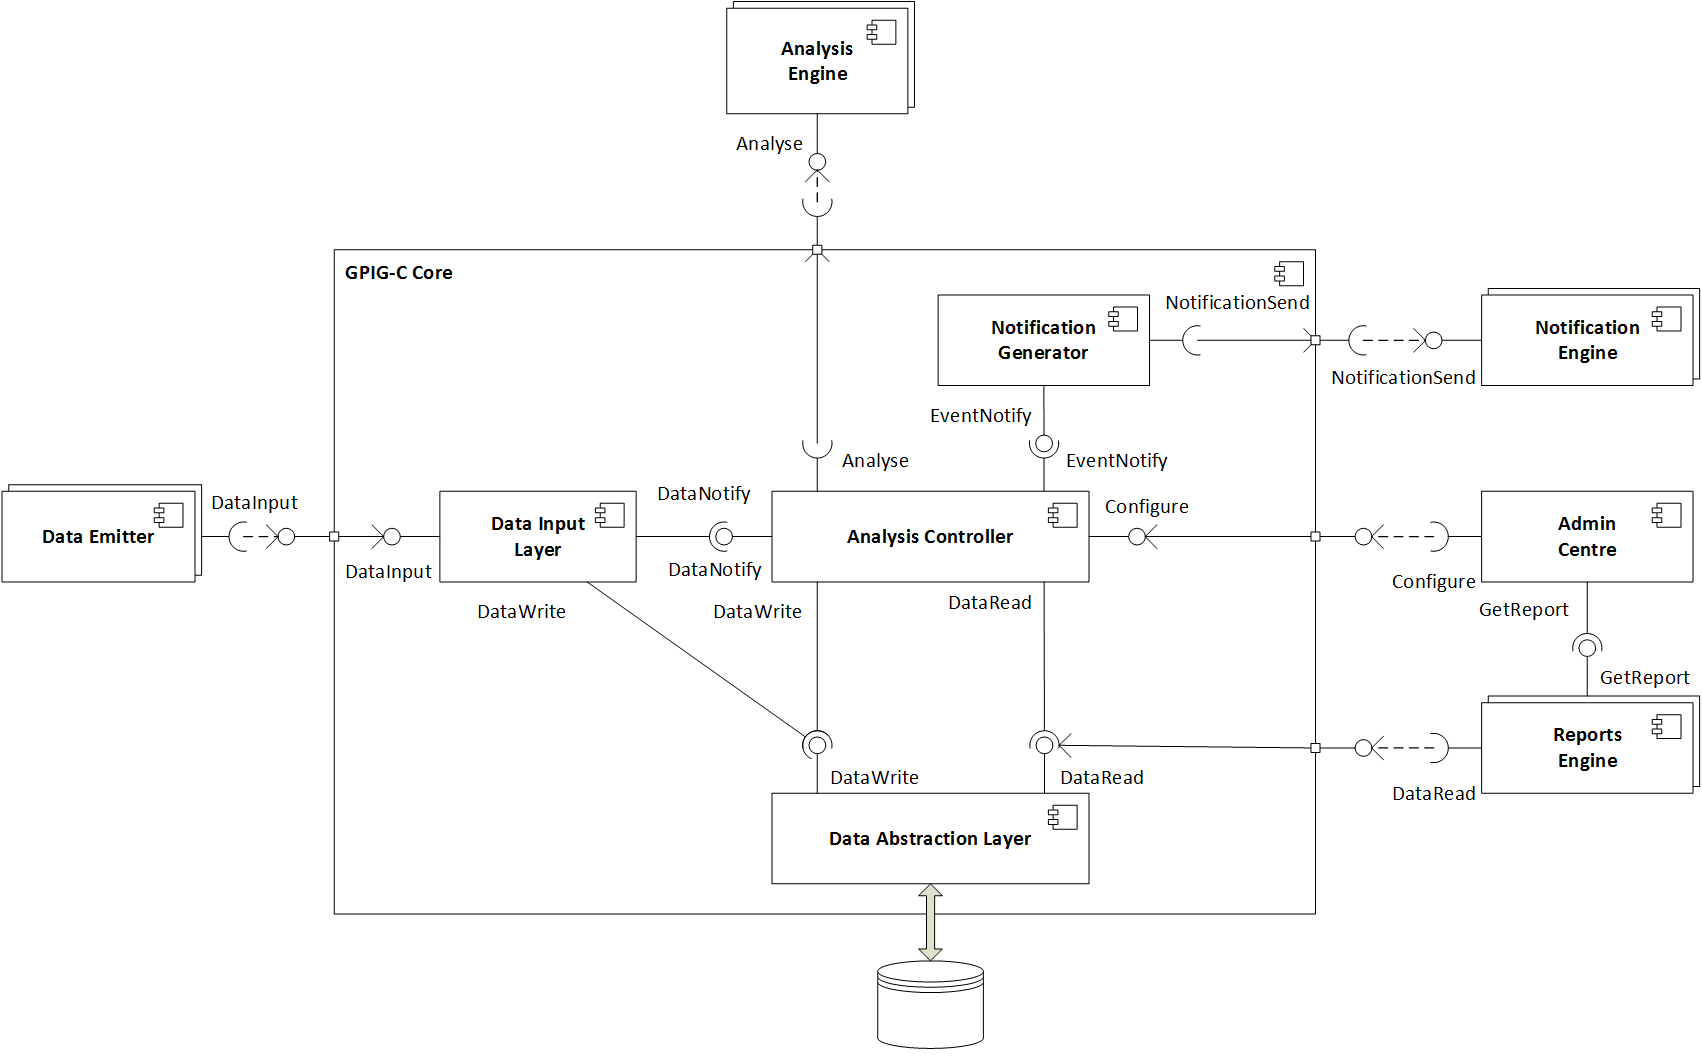
\includegraphics[width=14cm]{images/ComponentDiagram.png}
  \caption{The module diagram of the HUMS. Components shown in green are those provided as part of the GPIG-C system. Components shown in blue have default implementations provided as part of the system, but may be added to or replaced by the consumer.}
  \label{fig:ComponentDiagram}
\end{figure}

\begin{description}
  \item[Core] A collection of modules that must be run on a single machine, including the data input layer, analysis controller, data abstraction layer, and Notification generator. Additional modules can be integrated on the same machine or connected over a network interface.

  \item[Data Emitter] Sends data to the System core in a standard
    format. Should be tailored to the Consumer System it is extracting data
    from. May be part of the Consumer System itself.

  \item[Data Input Layer] Receives data from a Data Emitter and sends
    it to the data abstraction layer. Alerts the analysis controller
    that new data was received.

  \item[Data Abstraction Layer] Handles all interaction with the
    database, such that if the database were to be altered, only this
    layer would need to change.

  \item[Analysis Controller] Alerts analysis engines when new data
    has arrived, pulling the required data from the data abstraction
    layer. If an analysis engine determines an event has occurred
    within the data then the analysis controller forwards that event
    to the notification generator.

  \item[Analysis Engine] Analyses the data looking for trends. If a
    trend is found, an Event is returned to the analysis
    controller. Analysis engines will be included with the HUMS, but the
    Consumer may also provide custom engines.

  \item[Notification Generator] Receives events from the analysis
    controller, defines an abstract notification, and sends it to the
    appropriate notification engine.

  \item[Notification Engine] Receives an abstract notification from
    the notification generator and creates a concrete notification,
    for example an email or triggering a change in system
    behaviour. Notification engines will be included with the HUMS, but the
    Consumer may also provide custom engines.

  \item[Reports Engine] Pulls data from the data abstraction layer and
    formats it into a report, such as a PDF document or graph. Report
    engines will be included with the HUMS, but the Consumer may also provide
    custom engines.
\end{description}

\subsubsection{Behavioural View}

The module view shows how modules of the system are connected, but does not
however fully represent the interactions between components and the dynamic actions of the system. A behavioural view can be used to detail this information, showing the flow of data and events within the HUMS. Figure \ref{fig:CommunicationDiagram} shows a communication diagram of the 
HUMS, detailing how the HUMS receives data from a Data Emitter and generates a Notification. The different objects in the System are shown, along with all the interactions and links between them. The messages sent between different modules are shown and labelled with numbers to represent the chronological order in which they occur.

\begin{figure}[!ht]
  \centering
  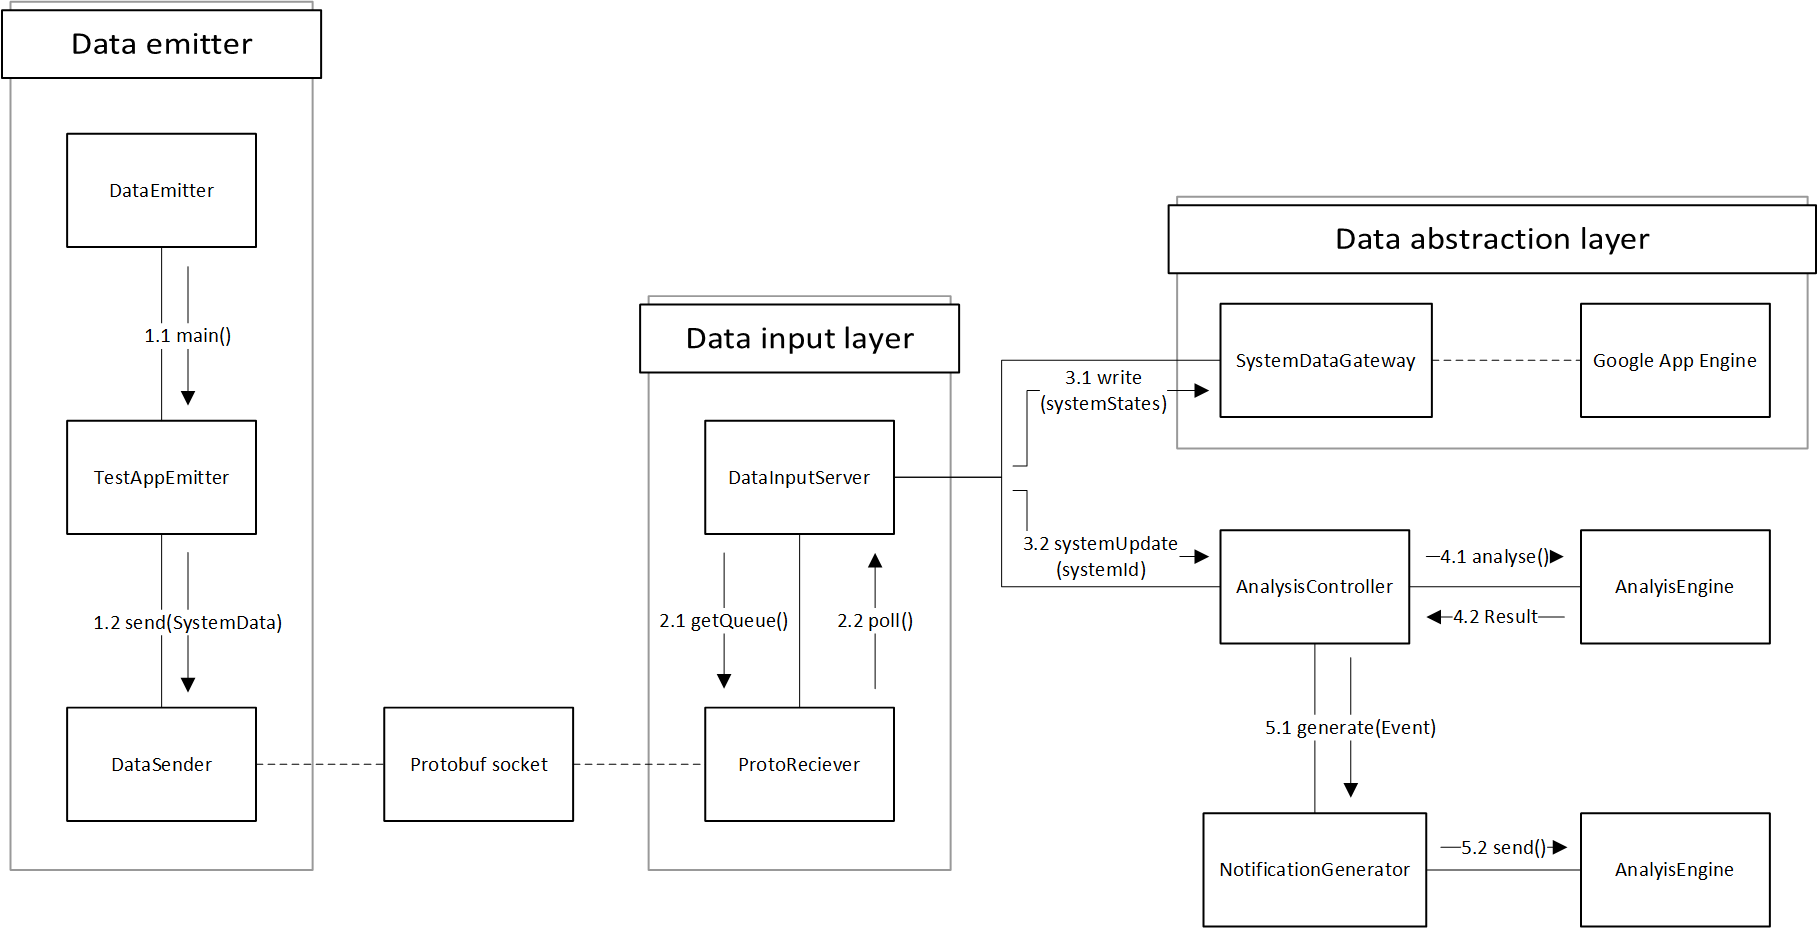
\includegraphics[width=14cm]{images/CommunicationDiagram.png}
  \caption{Communication diagram showing a behavioural view of message 
flow through the system, using UML 2 notation}
  \label{fig:CommunicationDiagram}
\end{figure}

\subsubsection{Execution View}
The HUMS needs to be tailorable to various deployment and execution strategies. The core system may be running on the same hardware as the Data Emitter or it may be geographically distant; engines may be on separate machines or may all be together. Figures \ref{fig:DeploymentDistributed} and \ref{fig:DeploymentIsolated} show the main scenarios for deployment of the HUMS, with a view that if the system architecture can perform under these situations, then it can perform under all others.

Figure \ref{fig:DeploymentDistributed} shows abstractly how the consumer system could be geographically distant to the HUMS core, engines and datastore. It also shows how a remote admin centre could be used, allowing configuration files to be created at a high level by business personel, as opposed to developers. This deployment possibility gave the team the idea of creating a system as a service (SaaS), whereby multiple customers can simultaneously use a single storage, analysis, and notification server. We felt this was an innovate addition to the HUMS concept as it removes some of the complexity for consumers in setting up and managing their systems, and allows the benefits of cloud computing to be utilised.

This deployment of our HUMS as a SaaS is shown in figure \ref{fig:DeploymentService}. For administering the HUMS as a service, a hosted admin centre will be created, allowing users to specify analysis and reporting behaviours using a simple rules engine-like interface. Users can define their own Events and how they should be handled, view all of the registered Clients, pull Reports, and view live visualisations of data.

Figure \ref{fig:DeploymentIsolated} shows how we envision the prototype HUMS being deployed at this stage, with all modules on the same machine. It also shows how the system will be deployed on an embedded system, with configuration files being created manually, without an admin centre, and all modules existing on the same device.

\begin{figure}[!ht]
  \centering
  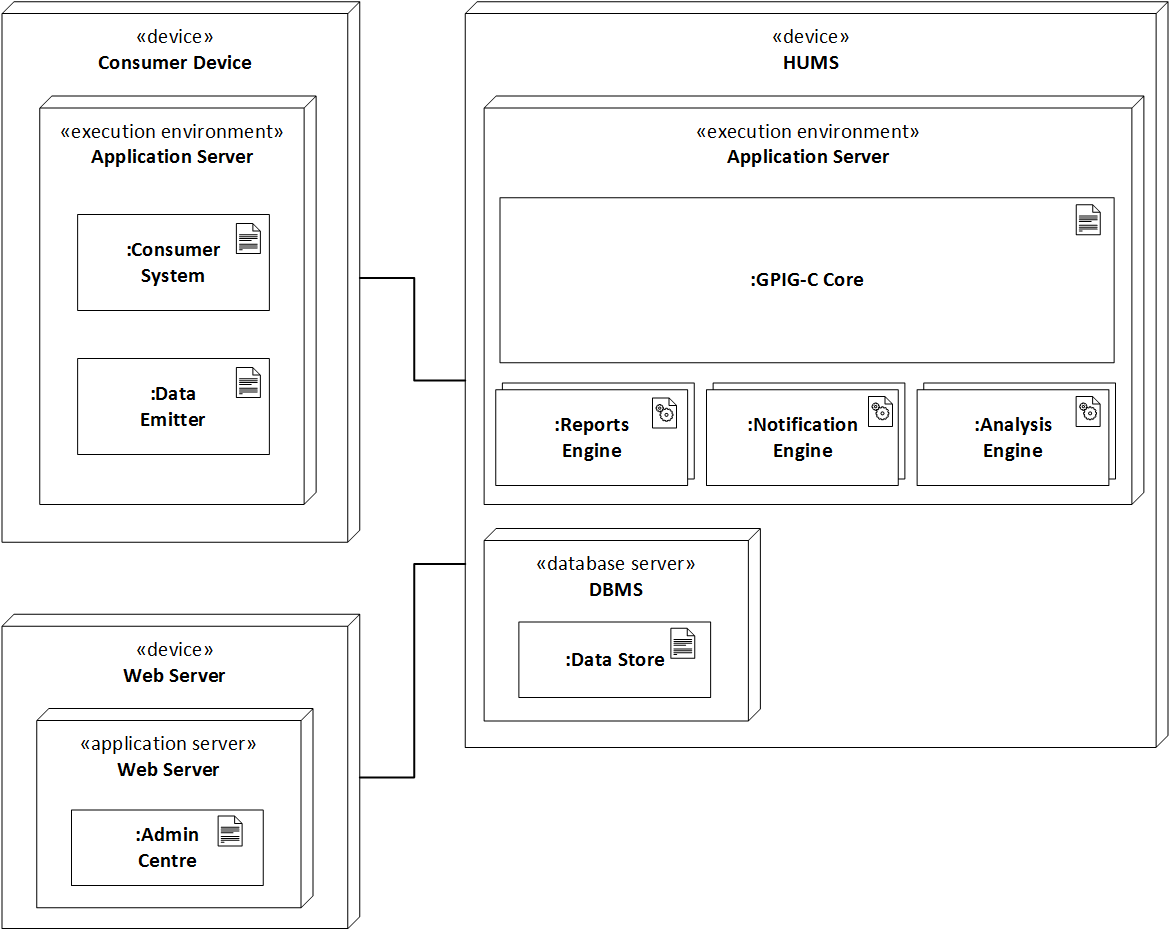
\includegraphics[width=10cm]{images/DeploymentDistributed.png}
  \caption{Deployment diagram showing the HUMS spread across multiple 
devices}
  \label{fig:DeploymentDistributed}
\end{figure}

\begin{figure}[!ht]
  \centering
  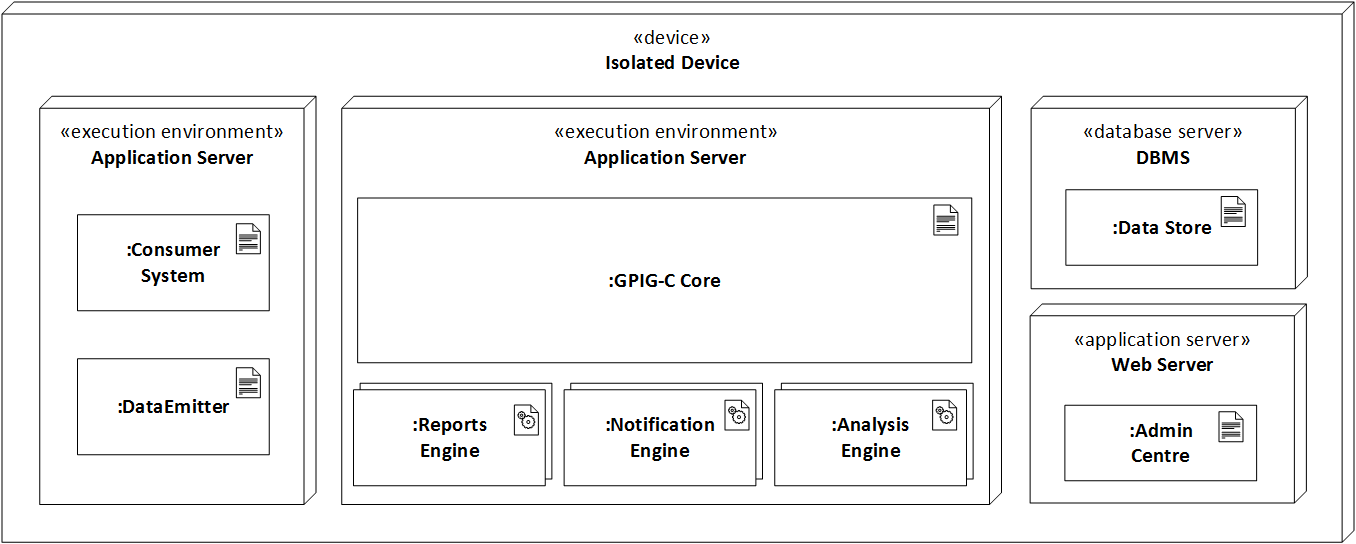
\includegraphics[width=12.5cm]{images/DeploymentIsolated.png}
  \caption{Deployment diagram showing the HUMS on a single isolated device}
  \label{fig:DeploymentIsolated}
\end{figure}

\begin{figure}[!ht]
  \centering
  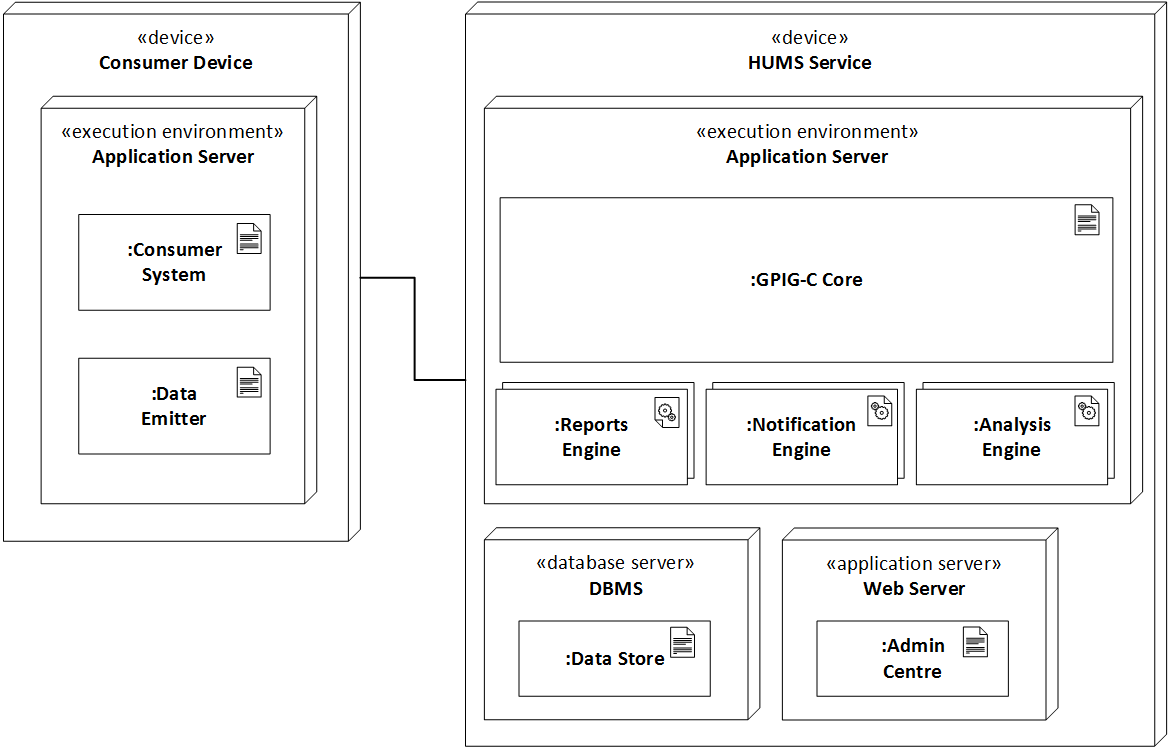
\includegraphics[width=10cm]{images/DeploymentService.png}
  \caption{Deployment diagram showing the HUMS as a multi-user service}
  \label{fig:DeploymentService}
\end{figure}

\subsubsection{Conceptual View}
The conceptual view is a description of the System in terms of its individual components, for example classes in an object-oriented design.

\subsubsection*{Data Input Layer}

The data input layer, shown in figure \ref{fig:dataInputLayer},
contains the following classes:

\begin{description}
  \item[DataInputServer] An object which starts a multithreaded
    server to receive connections, and periodically processes
    received data by sending it to the datastore and notifying the
    analysis controller. It accesses these by having references to them
    passed in upon creation.

  \item[ProtoReceiver] Listens on a socket for inbound connections,
    and then hands them off to a new ProtoMultiReceiver, running in a
    new thread, for processing. It also maintains a thread-safe
    concurrent queue, which all receivers write to, and the
    server reads (and removes) from. Use of multithreading
    enables multiple clients to send data at the same time easily, satisfying \nfrit{8}, and
    the use of a queue ensures that data is inserted into the database
    in the order in which it is received.

  \item[ProtoMultiReceiver] Receives data from a particular data input
    client, writing received data to the queue.
\end{description}

\begin{figure}[h!]
  \centering
  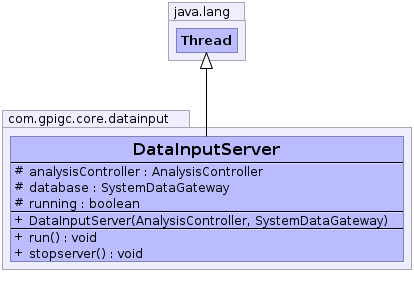
\includegraphics[width=6.2cm]{images/DataInputLayer/DataInputServer.png}
  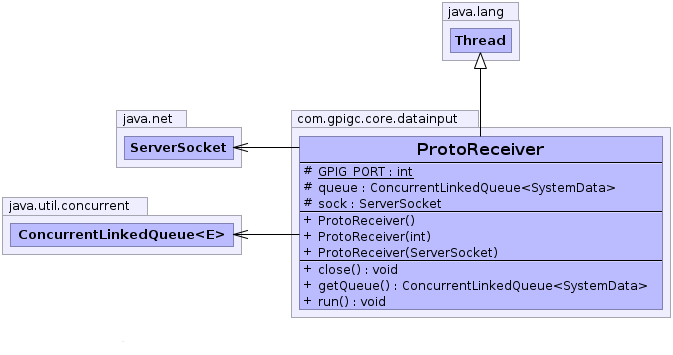
\includegraphics[width=8.3cm]{images/DataInputLayer/ProtoReceiver.png}
  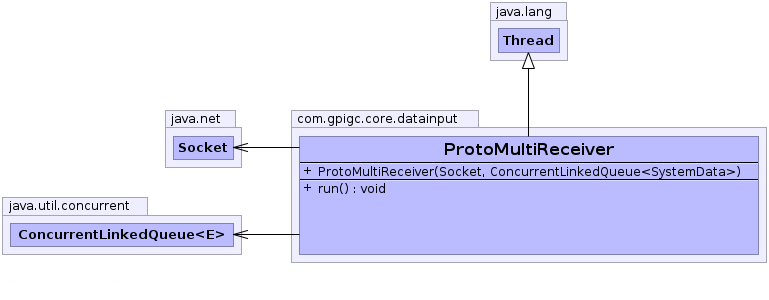
\includegraphics[width=9.5cm]{images/DataInputLayer/ProtoMultiReceiver.png}
  \caption{Conceptual diagrams of the data input layer classes in 
UML 2 notation}
  \label{fig:dataInputLayer}
\end{figure}

\subsubsection*{\hl{Data Abstraction Layer}} % TODO Looks like the stuff below

The data abstraction layer, shown in figure
\ref{fig:dataAbstractionPackage}, contains the following classes:

\begin{description}
  \item [SystemDataGateway] An interface used to abstract the
    datastore implementation details from the rest of the
    application. An implementation of this interface will provide ways
    to read and write from the chosen datastore, meaning the rest of the
    system is not concerned with the datastore implementation. When
    interfacing with a datastore, the end user will be required to
    implement this interface.

  \item [EmitterSystemState] An object representing the data received
    from a Data Emitter at a particular time. This object holds
    the System ID of the Consumer System and the creation timestamp along
    with a map of Sensor IDs against the value of the sensor at that
    particular time. A map was used to represent the sensors and
    values so that the Client is free to send data from any number of 
    Sensors at a time, reducing the number of writes to the
    database. For serialisation this object includes methods to
    convert to and from JSON.

  \item [DataJSONAttribute] An enumeration that wraps up the keys used
    to look up values in the JSON serialisations of the
    EmitterSystemState and QueryResult classes.

  \item [SensorState] An object representing the state of a particular
    system Sensor. A Sensor has a Sensor ID, a value and two timestamps. One
    timestamp specifies the time the Sensor value was added to the database and
    the other the time the actual value was sensed or created.

  \item [QueryResult] An object representing the result of a database
    query, containing the System ID of the Consumer System to which the
    data relates and a list of Sensor states pulled from the database.
\end{description}

\begin{figure}[h!]
  \centering
  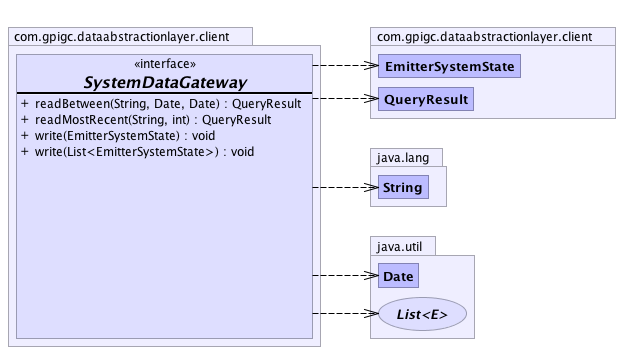
\includegraphics[width= 9.5cm]{images/DataAbstractionLayer/systemDataGateway.png}
  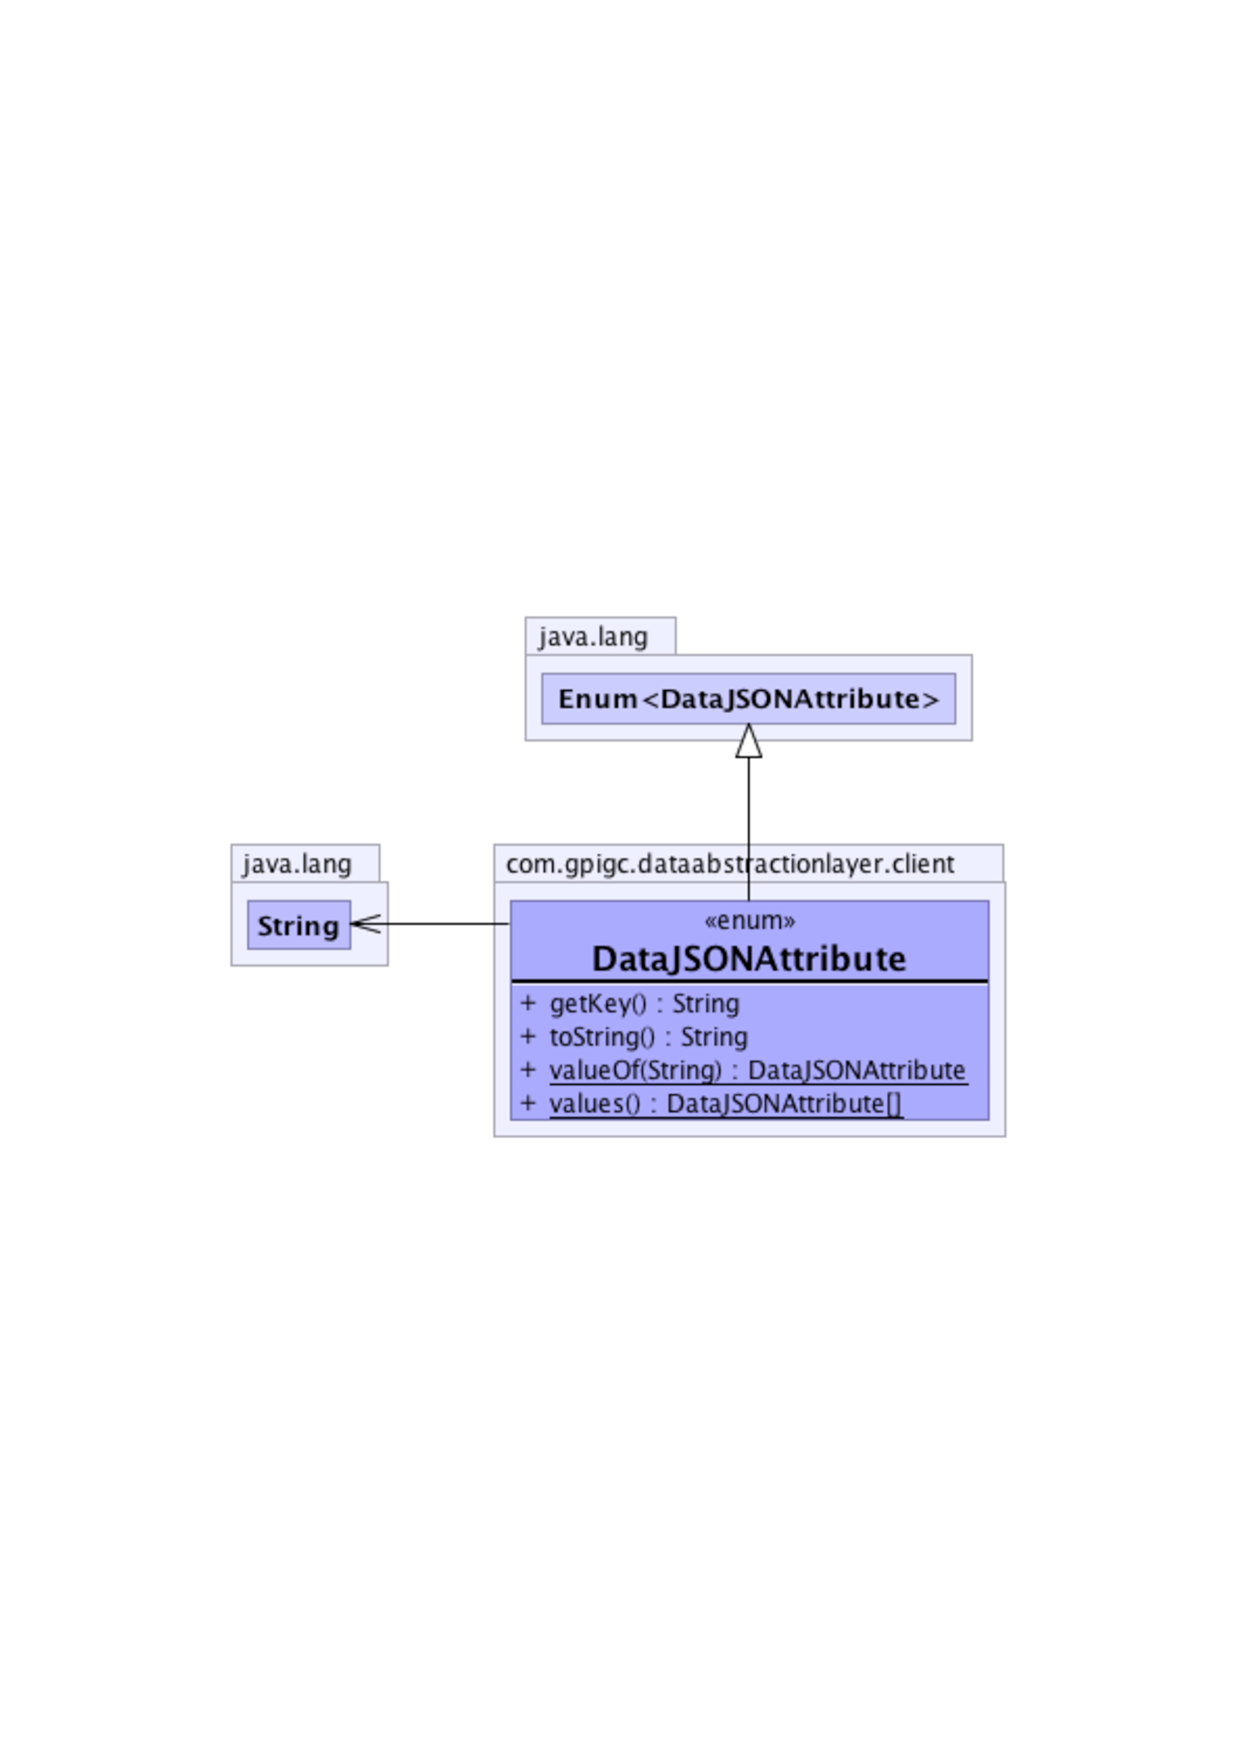
\includegraphics[width= 5cm]{images/DataAbstractionLayer/dataJsonAttribute.pdf}
  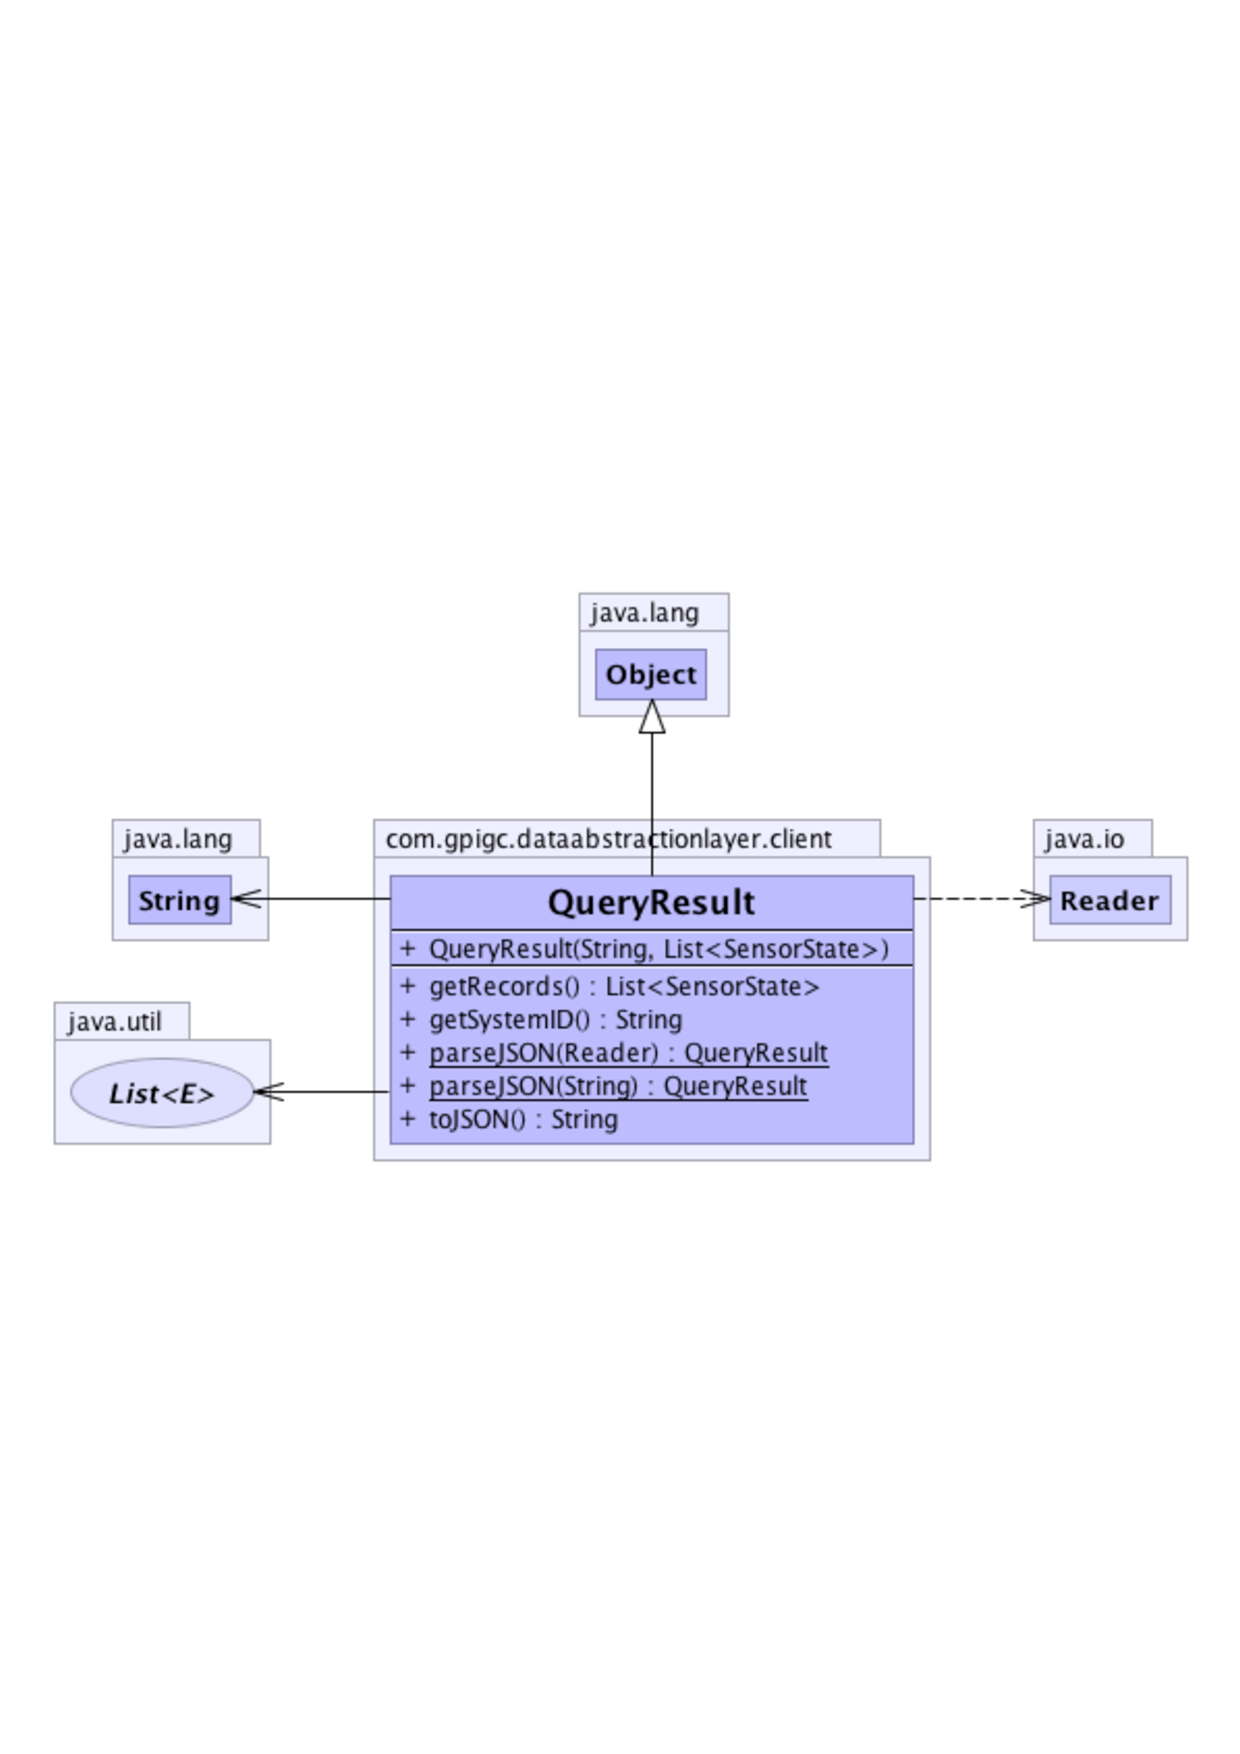
\includegraphics[width= 7cm]{images/DataAbstractionLayer/queryResult.pdf}
  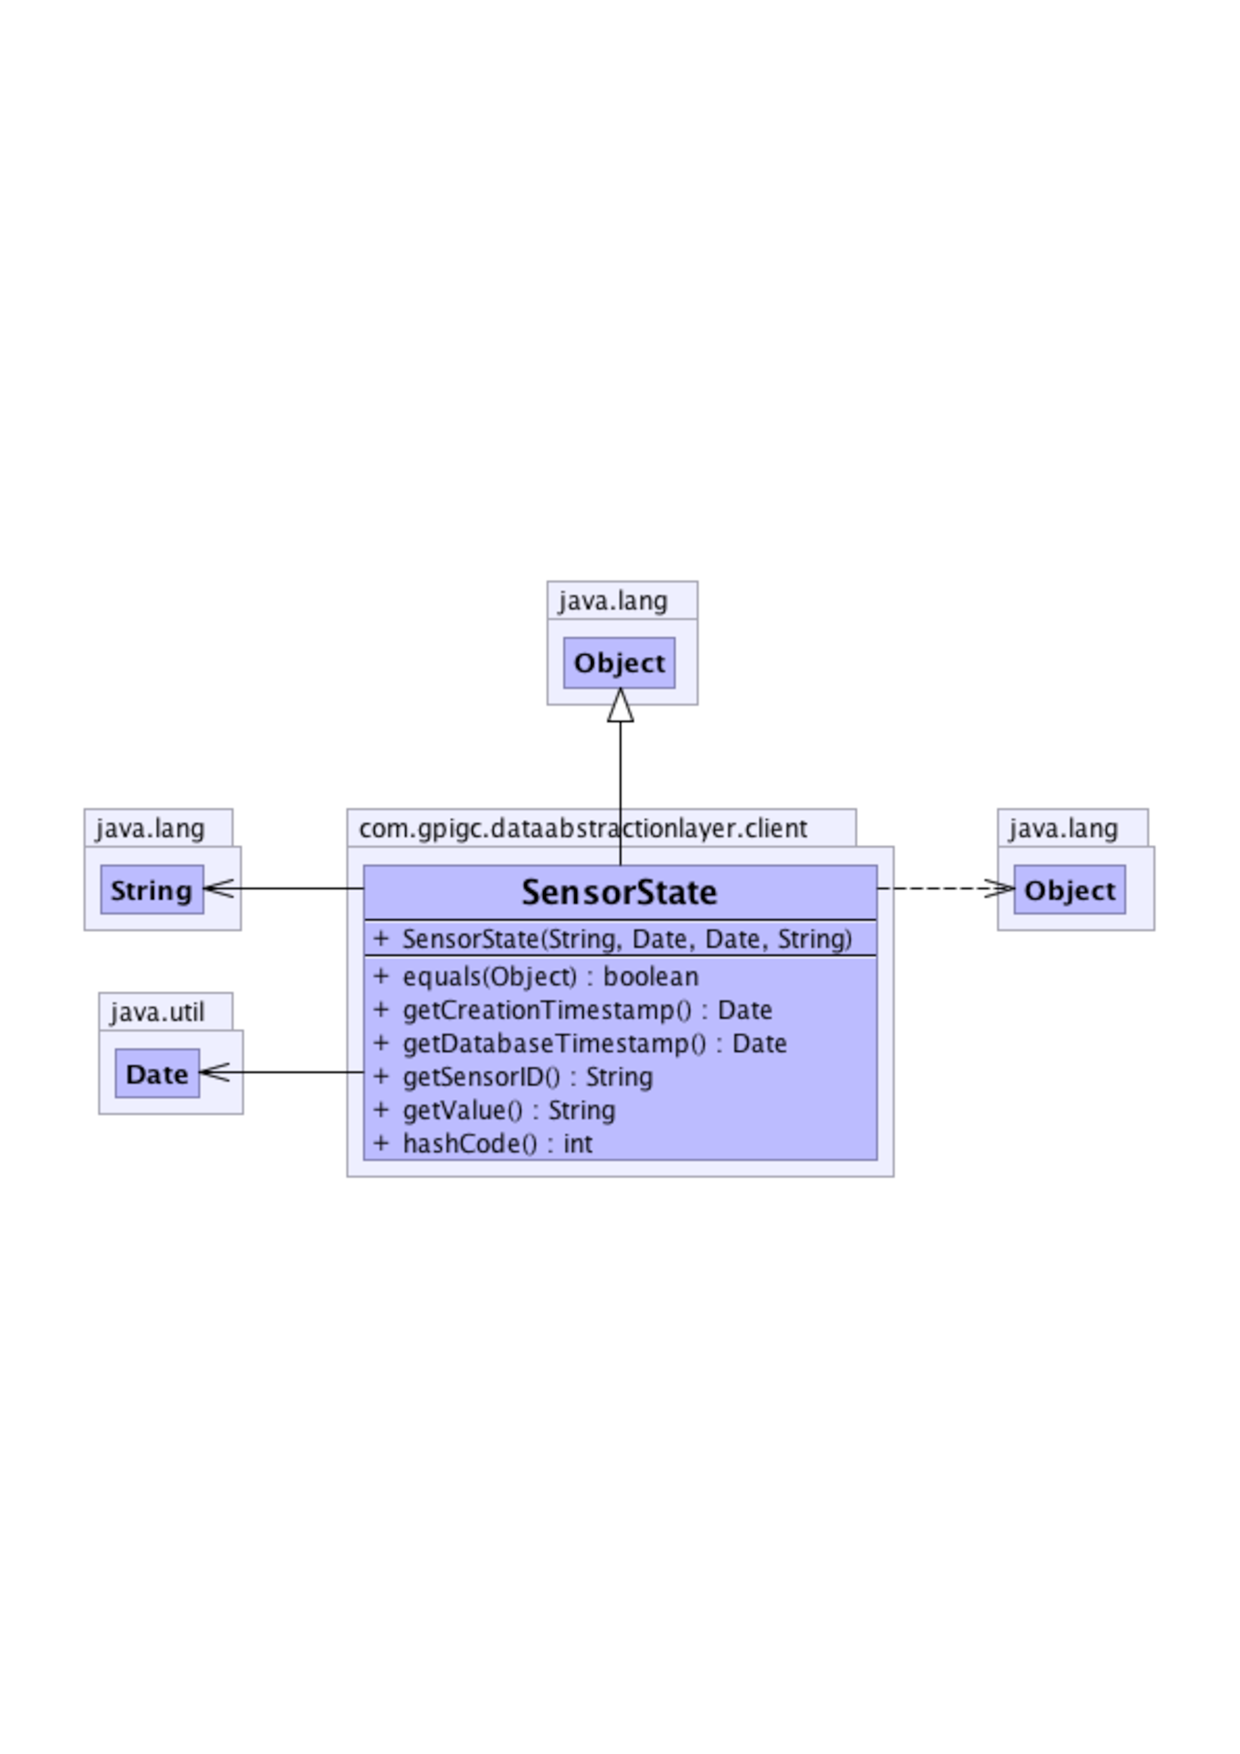
\includegraphics[width= 7cm]{images/DataAbstractionLayer/sensorState.pdf}
  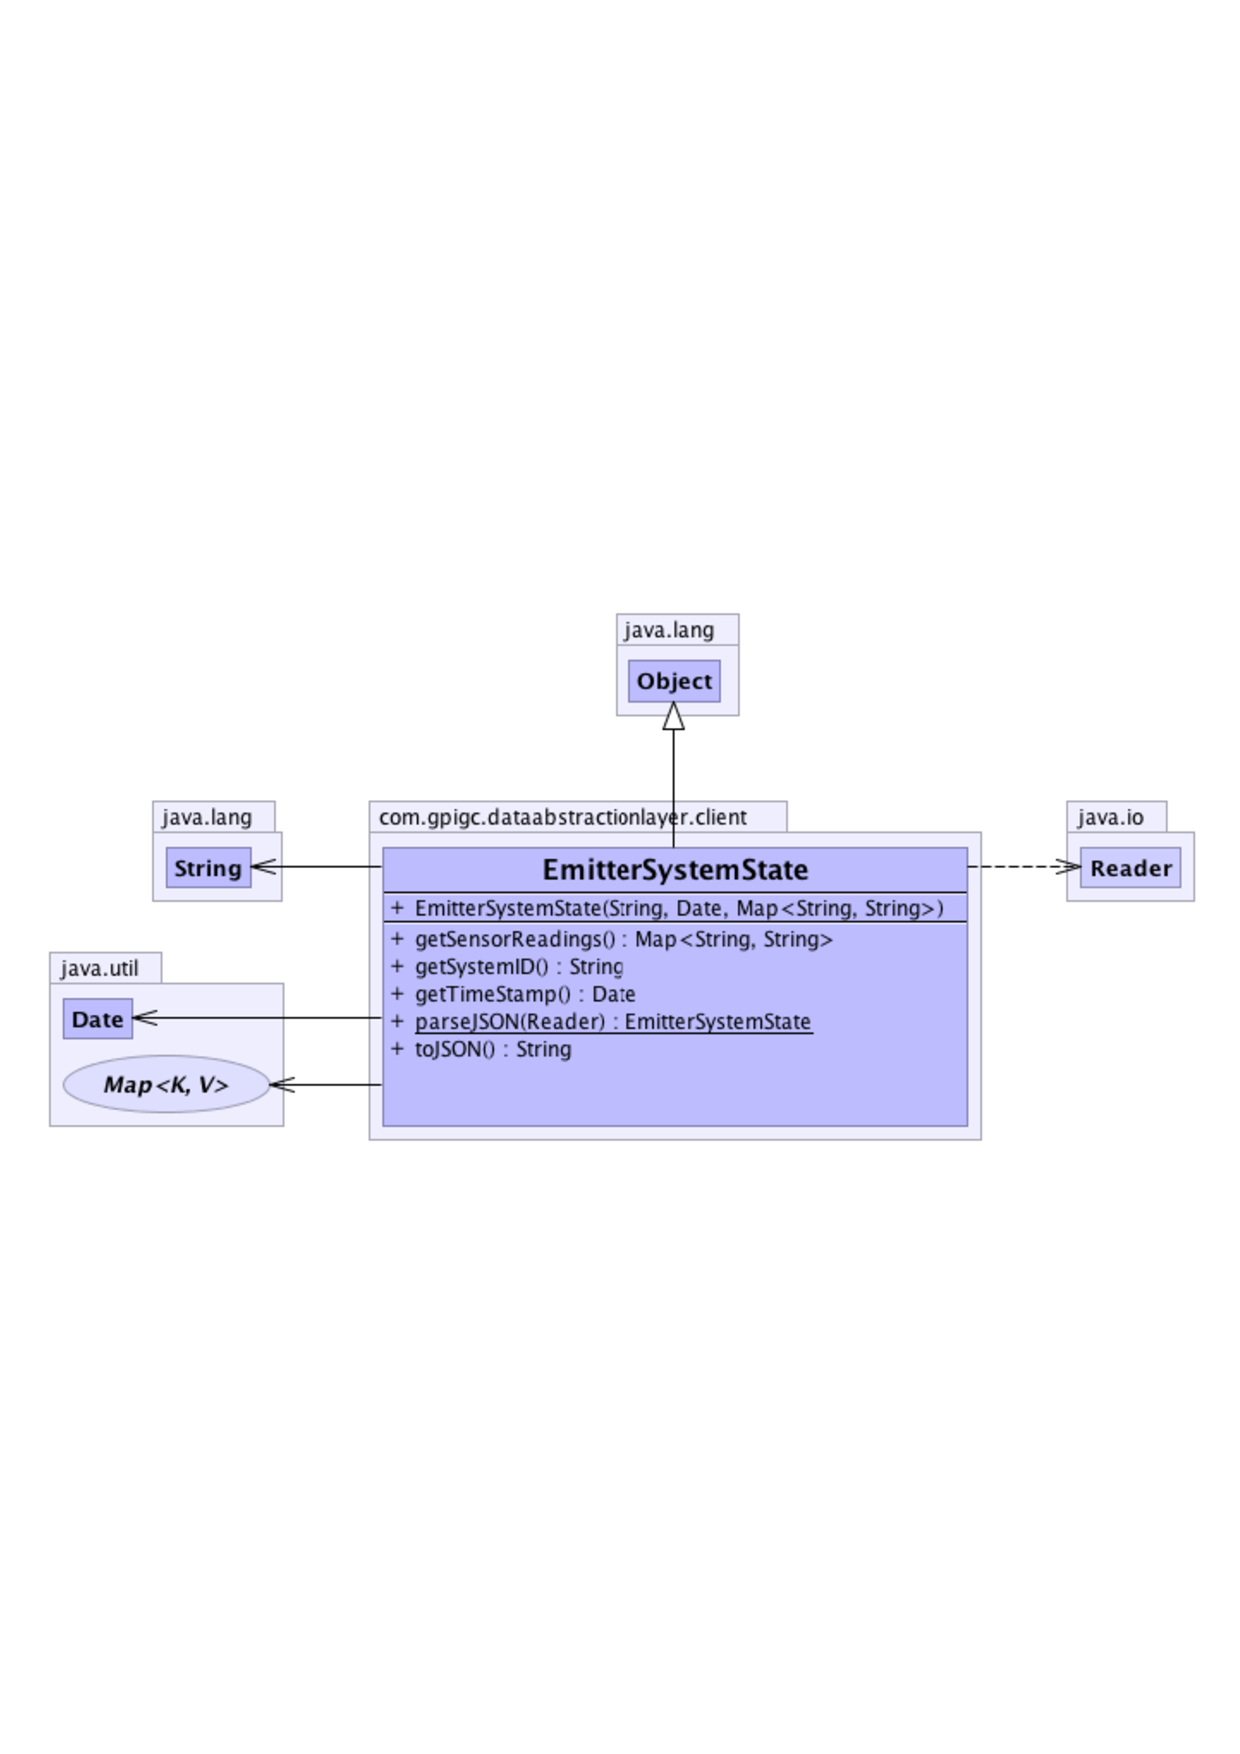
\includegraphics[width= 9cm]{images/DataAbstractionLayer/emitterSystemState.pdf}
  \caption{Conceptual diagrams of the data abstraction layer classes, 
using UML 2 notation}
  \label{fig:dataAbstractionPackage}
\end{figure}

\subsubsection*{Analysis Components}

The analysis components of the HUMS, shown in figure
\ref{fig:dataAnalysisComponent}, contain the following classes:

\begin{description}
  \item [AnalysisController] An object that coordinates all analysis of
    sensor data, interfacing with the data input layer by
    receiving a System ID when analysis is required. Once analysis is
    complete, the controller processes the results and triggers
    Notifications where appropriate. Analysis engines are associated
    with the analysis controller by class loading allowing for users to
    add and remove analysis engines at run-time.

  \item [AnalysisEngine] An abstract class that implements the basic
    functionality and defines the methods required of an implemented
    analysis engine. The \texttt{analyse} method interfaces with the database
    abstraction layer to retrieve the appropriate sensor data and then
    performs the desired analysis, returning a result object. When creating 
    their own analysis engines, the End User will be required to extend 
    this class, implement the abstract methods and define what 
    constitutes an Event.

  \item [MeanAnalysis] An analysis engine implementation which 
    computes a rolling average over values read from a Sensor over
    a given window. When called by the analysis controller, sensor 
    data is retrieved for all associated systems and mean analysis 
    is performed. If a mean value falls outside of the defined acceptable 
    bounds then a flag is set to generate a Notification.

% TODO DO we even need this object? Surely this is just an event
  \item [Result] An object representing the result of the analysis
    carried out by an analysis engine, containing a
    map between keys and values to be saved back to the database 
    and a flag indicating whether a Notification needs to be triggered.
    When implementing their own analysis engine the consumer will 
    be able to specify what data is to be saved back to the database.

  \item [Event] An object representing an Event,
    containing the name of the analysis engine that triggered the
    Event, the System ID of the Consumer System that the event corresponds
    to, and the result object from the analysis engine that triggered
    the event.
\end{description}

\begin{figure}[h!]
  \centering
  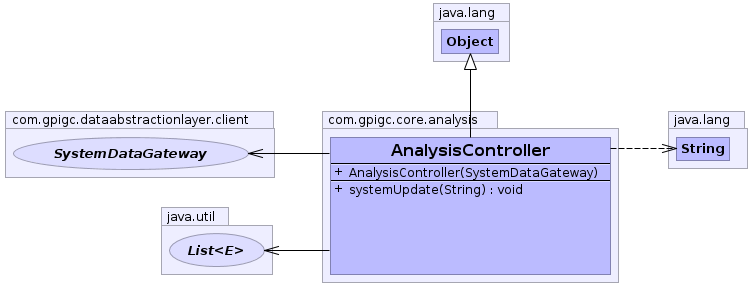
\includegraphics[width= 9.5cm]{images/Analysis/AnalysisController.png}
  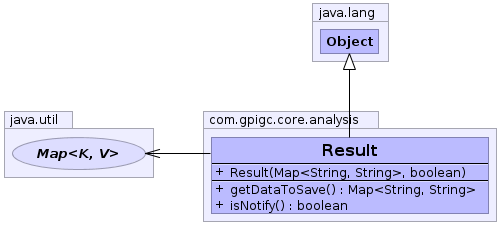
\includegraphics[width= 5cm]{images/Analysis/Result.png}
  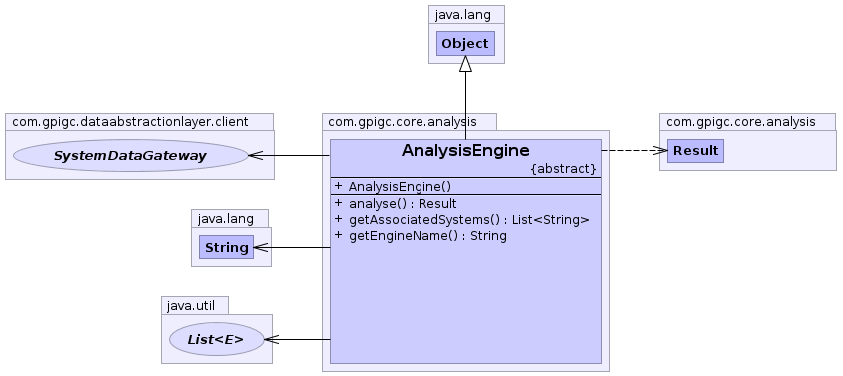
\includegraphics[width= 12cm]{images/Analysis/AnalysisEngine.png}
  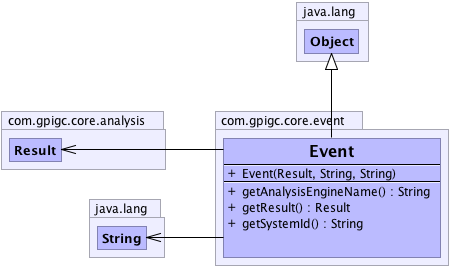
\includegraphics[width= 6cm]{images/Analysis/Event.png}
  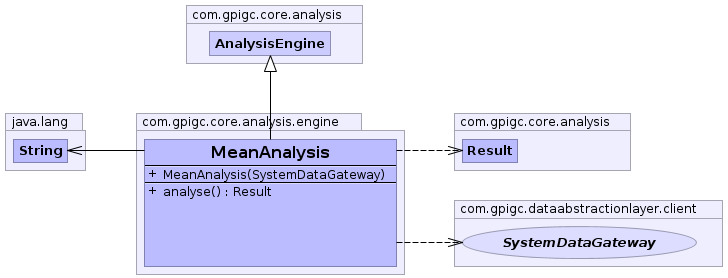
\includegraphics[width= 8cm]{images/Analysis/MeanAnalysis.png}
  \caption{Conceptual diagram of the analysis component classes in
UML 2 notation}
  \label{fig:dataAnalysisComponent}
\end{figure}

\subsubsection*{Notification Components}

The Notification components, shown in figure \ref{fig:notificationComponent}, 
contain the following classes:
\begin{description}
  \item [NotificationGenerator] An object that coordinates the generating and
    sending of notifications. The object interfaces with the analysis
    controller, receiving an event object when analysis engines specify that
    notifications should be sent. Notifications are then generated and sent by
    the registered notification engines. Notification engines are associated with
    the notification generator by class loading allowing for users to add and
    remove notification engines at run-time.

  \item [NotificationEngine] An abstract class implementing the basic
    functionality and defining that a notification engine instance must
    override. Notification engines feature a cool down system ensuring 
    notifications are not sent more then once during a specified period of 
    time.

  \item [EmailNotification] An extension of the notification engine
    class which notifies via email. When called by the notification
    generator, an email notification is sent to the specified recipient, 
    containing the notification subject and any further information.
\end{description}
 
\begin{figure}[h!]
  \centering
  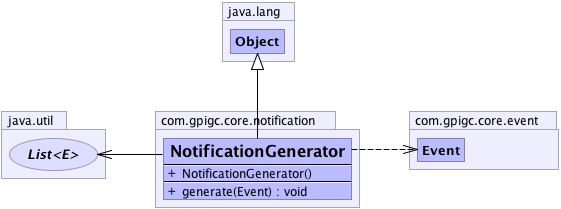
\includegraphics[width= 7cm]{images/Notification/NotificationGenerator.png}
  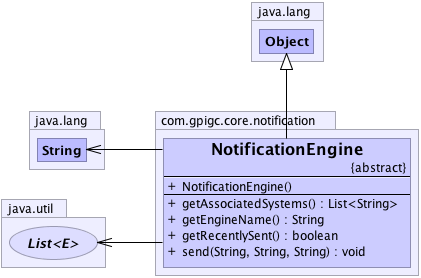
\includegraphics[width= 5cm]{images/Notification/NotificationEngine.png}
  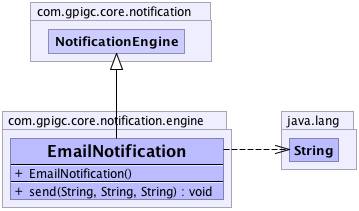
\includegraphics[width= 4.5cm]{images/Notification/EmailNotification.png}
  \caption{Conceptual diagram of the notification component classes in
UML 2 notation}
  \label{fig:notificationComponent}
\end{figure}

\section{Prototype Implementation}
\label{sec:prototype}

\subsection{Technologies}

We chose to develop the core of the HUMS prototype in Java. Java is typically
compiled to a bytecode that can be executed within a Java Virtual Machine (JMV).
Many environments support the Java Virtual Machine, including various
operating systems and the x86, x86-64 and ARM CPU architectures,
making it highly portable between desktop, server and embedded
systems \cite{javasupport}.

Whilst there may exist deployment platforms that are not supported, at
this stage, we do not see this as a problem since the underlying
architecture of the system is transferable to other languages.

All members of our team are familiar with the Java programming
language and thus no time was spent having to get the team up to speed
on a new language. We did not impose a language restriction when
developing the Data Emitter and various engines as the data being
passed between them and the core are language independent, meaning 
End Users are free, even with the prototype, to implement engines in any
language or with any tool they see fit. For the prototype, we used both Java and
JavaScript when creating the engines---languages that team members are
familiar with---allowing us to show off the versatility of the system.

For a particular example Consumer System used for testing (\hl{section}
\ref{sec:testapp}), it was required that the System monitor CPU and memory usage.
In order to do this, we began to investigate
technologies that provided this functionality, rather than reinvent the wheel.
Doing this also had the benefit of providing us with established, well-tested
tools with which we could easily implement data input Clients for further
systems. As the test program is a Java program, we had to connect to its 
JVM to query the heap usage, as the operating system would just report the 
size of the JVM heap. We settled on using SIGAR for process monitoring, 
and JMX for monitoring heap usage. An alternative we considered was 
simply querying the existing features provided by the operating system 
and JVM to access this data, however this would have not been portable 
across different operating systems, or to embedded systems with poor 
support for launching new processes.

To communicate between the core and the other modules, we serialised 
objects to send them over a network connection, using JSON and 
Protocol Buffers. For connections that require data to be serialised to text, 
we used JSON since it is human readable and maps well to our internal 
representation of objects in Java. To read and write JSON we used the 
Jackson library, since it offers a high-performance streaming API. When 
there was no such restriction on the format of the transmitted data, 
Google Protocol Buffers was used as it serialises objects to a binary format
that can easily be streamed to a TCP connection.
This performance may be necessary for the potentially 
high-volume connections between the Core and the other modules, 
such as Data Emitters and analysis engines. We initially considered 
using HTTP with JSON rather than Google Protocol Buffers for communication 
between the data input layer and the core, however we determined
that sending multiple HTTP requests a second would have significant 
overhead, and so we instead opted for a persistent connection and a 
more lightweight protocol.

We chose to use Google App Engine to host the prototype's database
module, displaying how easily it can incorporate existing, popular
datastore technologies. The prototype could easily be extended to
work with other database technologies simply by implementing an
interface within the data abstraction layer. Google App Engine was chosen
as opposed to a local datastore as it allowed for the prototype to
easily interface with the admin centre.

We created a prototype admin centre to show how the HUMS could be
managed remotely, viewing data and modifying settings online through
a web browser. The admin centre, shown in figure \ref{fig:admin} was
developed using the Bootstrap front-end web framework, in order to create
a prototype realistically simulating an interface to the HUMS that is accessible
on desktop computers, laptops and mobile devices alike.

\begin{figure}[h!]
  \centering
  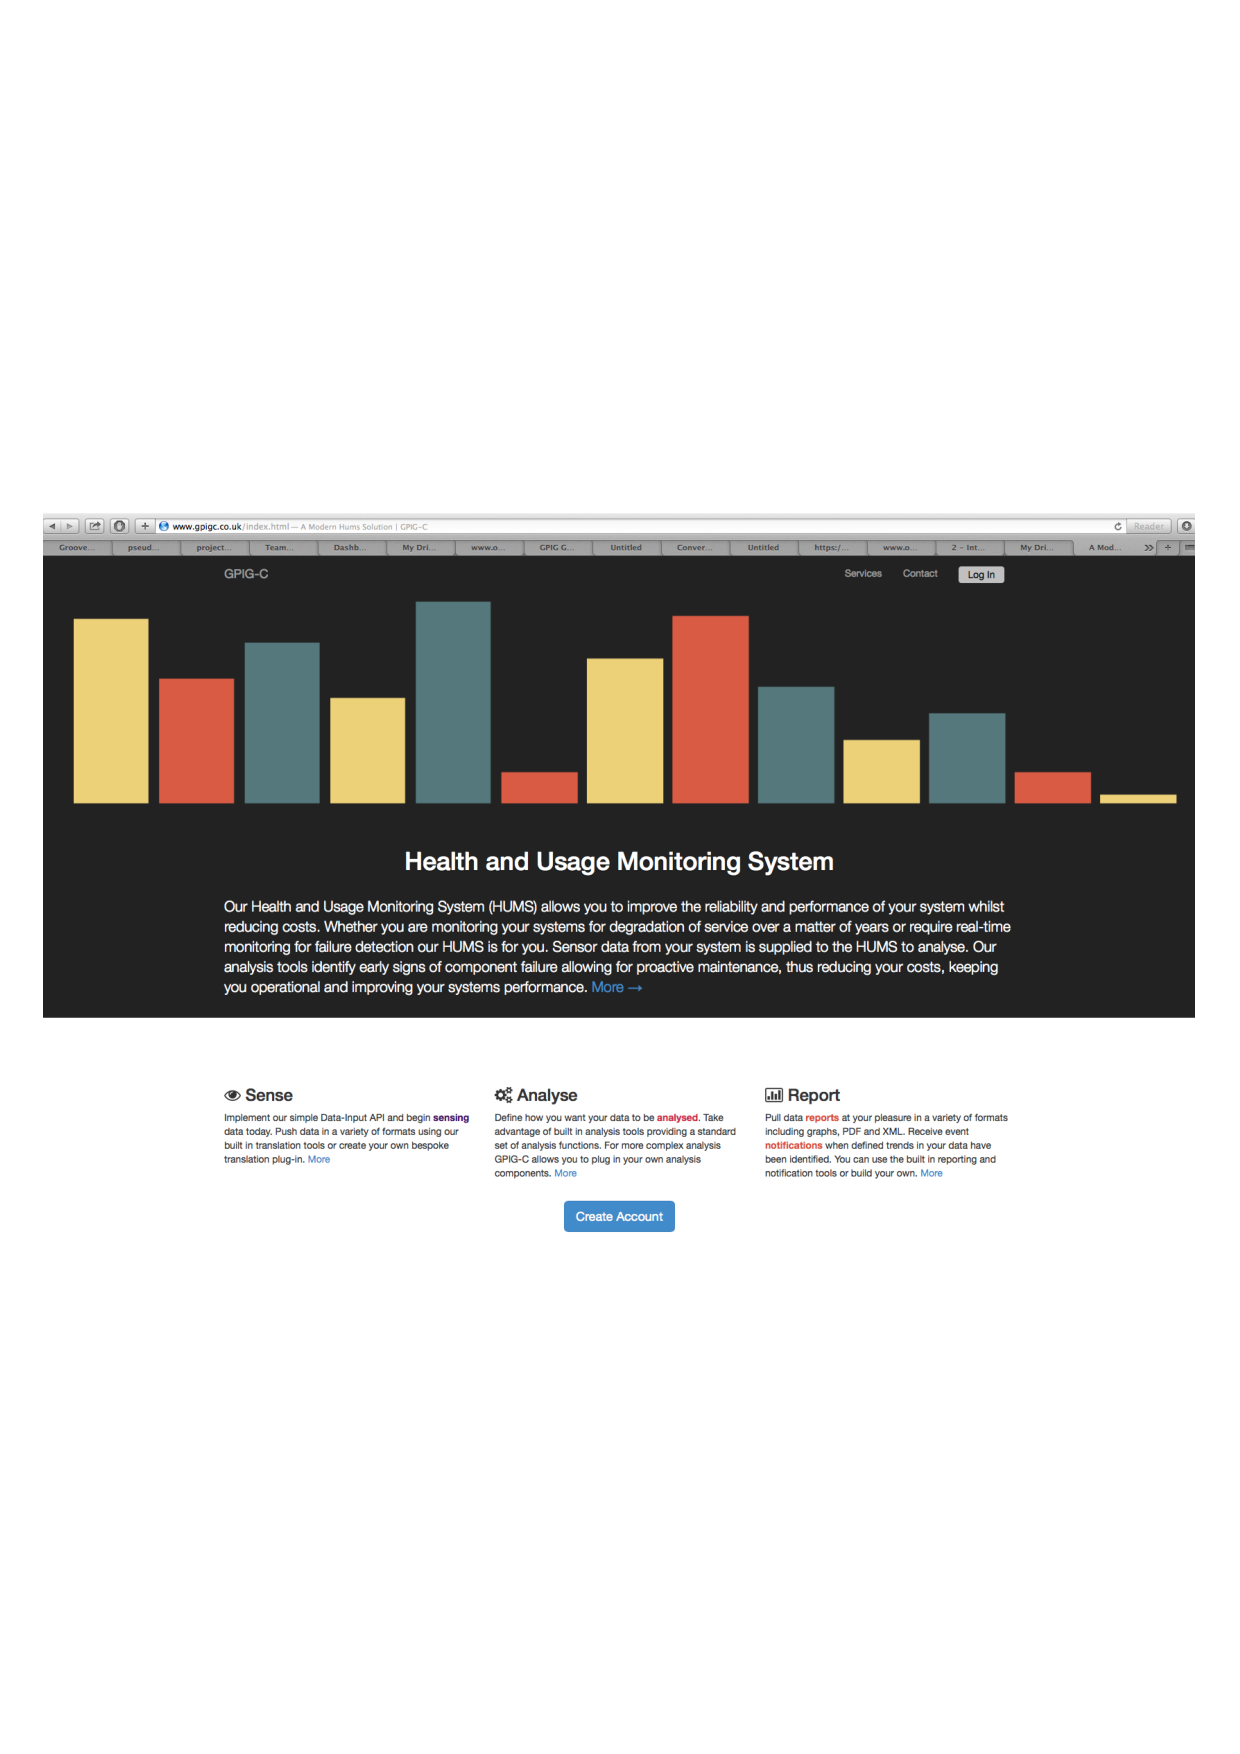
\includegraphics[width=15cm]{images/admin.pdf}
  \caption{A screenshot of the admin centre homepage}
  \label{fig:admin}
\end{figure}

We used various Java libraries to support our prototype, saving us 
development time and providing a robust codebase. For testing we used 
the Mockito framework to allow us to verify elements of our codebase in 
isolation, by offering a concise way to mock out dependancies.

We used Git for version control, allowing the entire team to
contribute to the project simultaneously, whilst keeping a reversible
history of all alterations made by each person. We considered using a
centralised version control system, such as Subversion, but decided that the
benefits provided by a decentralised system, such as Git, for working
independently and then combining work would outweigh the potential
disadvantages of there being no managing server. As we used GitHub for the
canonical copy of the repository, we incorporated many of the benefits of centralised
version control anyway.

\subsection{Current Functionality}
For the interim prototype, we chose to firmly follow the planned architecture, producing a core system linking to example engines, Data Emitters and data stores, focussing on interacting with the provided test application.

The core of the HUMS is fully functional, allowing for Data Emitters to send data 
to the data input layer using Protocol Buffers, chosen in preference to HTTP 
requests due to the lower latency. The data input layer, as currently 
implemented, supports multiple simultaneous connections from input clients, 
although we have yet to investigate how many the prototype could handle. 
Upon receipt, the data is put into a queue, which is periodically processed by 
the data input server, by adding each entry to the database and notifying the 
analysis controller. The analysis controller allows for dynamic loading of 
analysis engines, allowing them to be altered at runtime and requests data to 
be passed to the appropriate engine, decoupling the analysis engines from the 
data abstraction layer. The data abstraction layer provides a simple interface to 
be implemented by the Consumer and includes an example implementation, 
interfacing with Google App Engine using HTTP requests to a remote servlet. 
The Notification generator also allows Notification engines to be dynamically 
loaded and passes Event objects to them.

Currently there are two Data Emitters for use with the HUMS, demonstrating its 
flexibility. The first extracts and emits data about the JVM, recording CPU and 
memory usage, and the second extracts and emits live data about earthquake 
activity from the USGS earthquake hazards program API \cite{usgs}.

The Data Emitter designed to emit data about the JVM records the CPU and 
memory usage of the application and sends these through the data input API 
every second. A period of four seconds is allowed to elapse before the first 
send, allowing the CPU usage readings to stabilise. The Data Emitter created to 
relay live data about earthquake activity fetches data every minute from the 
USGS earthquake hazards program API and submits it to the data input API.

%%Paragraph about analysis plugin 

When the notification generator receives an Event, it selects the appropriate 
notification engines for that Event and uses them to create and send  
Notifications. Currently, a single notification engine has been developed which 
sends an email to an email address configured by the User. This is 
demonstrated for the test application, where an email will be dispatched when 
CPU usage exceeds a predefined limit.

A prototype admin centre was created for this stage of the project to 
demonstrate how the HUMS could be public facing as a SaaS, allowing for any 
company or individual to, for a fee, use the facilities provided. This service includes
storage, analysis, notification, and reporting tools. Currently the prototype 
admin centre mocks functionality and --- apart from the reporting examples --- 
does not actually integrate with the system. We envisage that in the next phase 
of the project the admin centre will be fully functional and will interact with the rest of the HUMS modules where appropriate.

We chose to add our reporting tools to the admin centre in the form of a map
and a graph, each of which is updated live, to be used with test applications as shown in figures~\ref{fig:alerting} and~\ref{fig:graphing}.

\subsection{Source}
\label{sec:source}
The source for our prototype implementation can be accessed online at \texttt{http://git.gpigc.co.uk} and cloned using Git from \texttt{http://git.gpigc.co.uk/gpig-c.git}. The username and the password hint are \texttt{gpigc} and ``It's right under your nose''\footnote{Password is \texttt{moustache}}.

\subsection{Prototype Evaluation}
\label{sec:prototype-evaluation}

\subsubsection{Customer Test Application -- No. 1}
The customer provided an example application to monitor as part of the
evaluation of our prototype. With this in mind, we created a monitoring 
package for our prototype solution that can monitor a native application
or one executing on the JVM. We utilised Java Management 
Extensions (JMX) to sample the memory utilisation of the application and
created a process monitoring class which monitors the total
CPU usage of the application. The mean analysis engine computes a 
rolling average of values, and causes an email to be sent if this value
becomes too high, as shown in figure \ref{fig:alerting}. The raw memory
values are read by the reporting system and displayed live in the admin
centre, as shown in figure~\ref{fig:graphing}. The graph shows a value from
every 10 seconds, and automatically updates with the latest values.

\begin{figure}[h!]
  \centering
  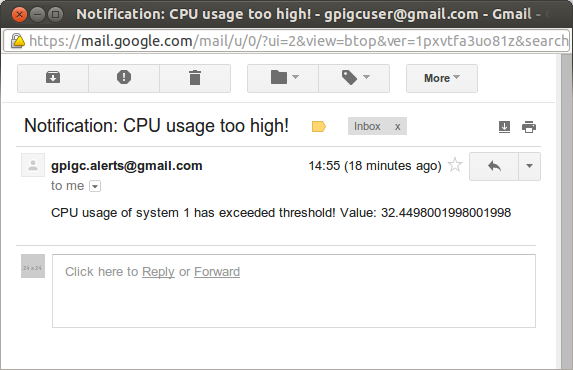
\includegraphics[width=7cm]{images/TestApplicationCPUAlert.png}
  \caption{A screenshot of an email notification sent by the mean analysis engine}
  \label{fig:alerting}
\end{figure}

% TODO Talk about performance or meeting the requirements - we've not implemented quite a few things such as feedback?

\begin{figure}[htbp!]
  \centering
  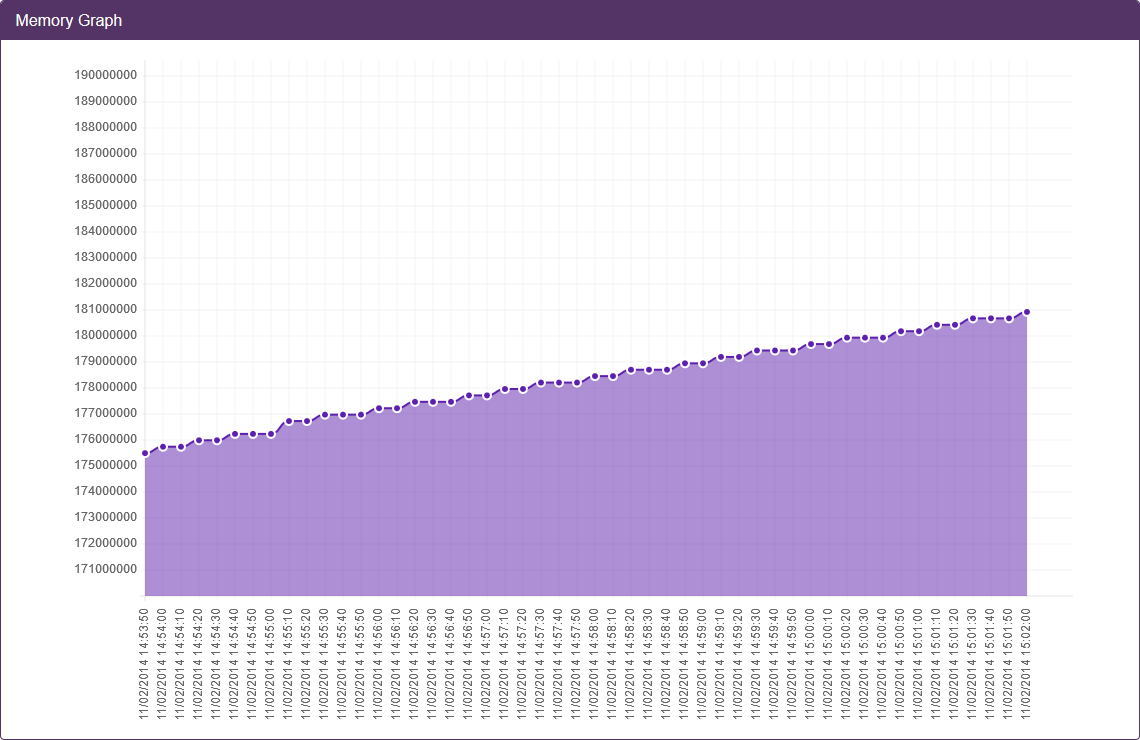
\includegraphics[width=12cm]{images/TestApplicationMemoryGraph.png}
  \caption{A screenshot of the live graphing of the memory usage of the Customer 
  Test Application}
  \label{fig:graphing}
\end{figure}

\subsubsection{Earthquake}
We also created our own sample application: monitoring earthquakes 
through the USGS Earthquake Hazards Program API. The HUMS
can collect live data from the API, store it and plot the location of any
detected earthquakes on a map of the world in the admin centre, as shown
in figure~\ref{fig:plotearthquakes}. We felt that using a map to display
data was a useful and innovative addition.

\begin{figure}[h!]
  \centering
  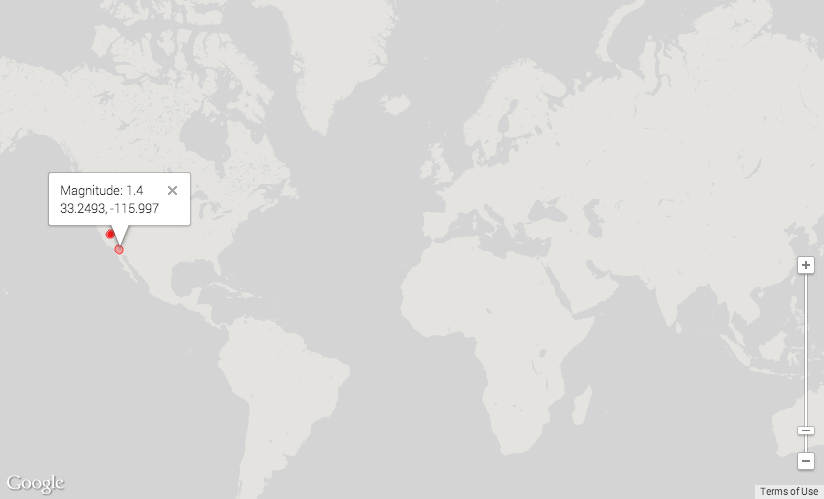
\includegraphics[width=10cm]{images/plotearthquakes.png}
  \caption{A screenshot of the admin centre for our live earthquake monitoring HUMS prototype}
  \label{fig:plotearthquakes}
\end{figure}

\subsubsection{Instructions for Running and Replicating Results}
We have compiled and packaged our source code into an easy to run distribution, which can be obtained from \hl{FIX}\verb+http://www.gpigc.co.uk/dist.tar.gz+. The user name and password to access this and any other resources on this domain is the same as described in section \ref{sec:source}.

Once extracted, the shell script \verb+launch.sh+ can be run to correctly start the different components and the Customer Test Application. At this stage the distribution only runs on Linux-based systems. This is because development was primarily conducted on Linux, and a lot of target systems for the HUMS are Unix based. Running from source works successfully across multiple platforms so in future we expect to create a distribution which can also do this.

An additional shell script named \hl{FIX}\verb+launch-eq.sh+ exists to run the components of the system with our own earthquake monitor test application. An internet connection is required for this to run as the data is accessed from an online source.

Data collected from the Customer Test Application can be observed at \texttt{http://www.gpigc.co.uk/\\*admin/map.html}, and data collected by our earthquake monitor can be observed at \texttt{http://www.\\*gpigc.co.uk/admin/graph.html}.

\subsection{Testing} 
We created and implemented a test plan that laid out our key ideas
with respect to verifying that our solution fulfilled its
requirements. In this section we give the mapping between each
test and its associated requirement. We
defined our plan, where appropriate, in terms of each module within
the system and what specific, testable attributes that module must
have to fulfil its requirements. We also further deconstructed the
testing into various levels of abstraction, mapping the higher level
requirements to their lower level requisite requirements: acceptance
testing, system testing, integration testing and unit
testing.

% TODO We probably need something about overall system & acceptance
% testing. These are mainly the white/black/grey box tests in the
% first report, e.g. NRF.9, "The system must cope with up to 2000 data
% input re- quests per second per HUMS instance."
% Also talk about what we can't test since not everything is implemented

For system testing, we completed inspection testing, and deployed our system across various networked machines and verified that the HUMS acted as expected. A more thorough system testing stage will be completed for later, higher fidelity, iterations of the prototype.

For acceptance testing, we sent the customer various iterations of our prototype, and we expect that the feedback from this report will fold back into our acceptance testing.

Below, the testing within each module is described:

\begin{description}

% TODO Verify the requirement IDs in the section below
  \item[Data Emitter] The purpose of the data emitter is to run
    continuously, monitoring a system and reporting on it, thereby
    fulfilling \frit{1.2}. We completed inspection testing to verify 
    that data was reported, along with running the program for 
    several hours to verify that it continued to function.

  \item[Data Input Layer] For the data input layer, it is essential that large
    amounts of data can be received in parallel. We verified this by
    inspection testing, and also by running multiple clients simultaneously and
    verifying that the data from both was recorded, thus verifying \frit{1.1}.

  \item[Data Abstraction Layer] Given the high throughput and
    importance of storage to the function of the HUMS as a whole, the
    data abstraction layer's key attributes are availability and
    performance. We completed an inspection test and used the 
    GWTSystemDataGatewayTest class to verify \frit{3.1}. At the unit 
    testing level, as  part of TDD, we focussed on the comparably complex,
    well defined module-internal functions, such as the generation and 
    parsing of the JSON serialisation of objects.
    
  \item[Analysis Controller] Due to the central role played by the 
  analysis controller in the analysis pipeline we identified its key 
  attributes as performance and testability. We utilised Mockito to 
  provide completely isolated unit tests, confirming that notifications 
  are only triggered when appropriate, satisfying \frit{7} and \frit{9}, and 
  that only the relevant analysis engines are used for a given system, 
  satisfying \frit{7.3}. Class loading was used to load analysis engines for 
  the prototype, this was confirmed to be working via inspection and 
  integration testing.
  
  \item[Analysis Engine]
   For the analysis engine, we created a unit test to check each aspect of the 
   engine as per \frit{7.1} and \frit{7.4}. Again, we utilised Mockito to mock out
   dependancies, restricting the possible sources of failure of a test to be 
   as narrow as possible. This was especially useful for potentially flakey 
   areas, such as database access or connecting over a network that may 
   not be available at test time. Our unit tests covered valid, extreme and 
   null values being sent to the analysis engine.

  \item[Notification Generator] For the notification generator, we created 
	multiple unit tests to verify functionality as per \frit{8}. Mockito was 
	used to isolate the class, allowing for a true unit test. The initial 
	test ensured that a notification is generated when analysis has indicated 
	it. The second test ensured that notifications were only sent once, to 
	avoid spamming users.	 
  
  \item[Notification Engine] The functionality of the email notification 
	engine is tested using a unit test. The test uses the notification engine 
	to send a message to a certain recipient with a given subject and
	message, then verifies that the email was successfully sent and 
	received by checking the inbox of the specified recipient and 
	inspecting the message to ensure that it contains the correct 
	information, satisfying \frit{9}.

  \item[Reports Engine] We tested the Reports Engine by inspection since it 
	is a prototype and does not require significant automated testing at this 
	stage.

 \end{description}

\subsubsection{Traceability Table}

Table~\ref{tab:traceability} shows the existing tests used to verify the implementation of the requirements in the system.

\begin{table}[H]
\centering
\begin{tabular}{| p{1.5cm} | p{5cm}| p{1.8cm}| p{4.8cm}|}
  \hline\rowcolor{titleColor} \textbf{Req. ID} & \textbf{Test Classes} & \textbf{Type} & \textbf{Details}\\
  \hline \fr{1.2}   & N/A & Inspection, Alpha & Verify by observing output in admin centre\\
  \hline \fr{2.1}   & SystemDataTest & Unit & Verify existence of timestamp\\
  \hline \fr{2.2}   & EmitterSystemStateTest & Unit & Verify existence of timestamp\\
  \hline \fr{3}   & SystemDataTest,\newline EmitterSystemStateTest,\newline QueryResultTest & Integration, Unit & Read and write to database, create and parse JSON\\
  \hline \fr{7.1}   & AnalysisControllerTest, \newline NotificationGeneratorTest & Inspection,\newline Unit & Check notification flag is set and queried to control notifications\\
  \hline \fr{7.4}   & AnalysisControllerTest & Unit & Verify generation of events \\
  \hline \fr{11}    & EmailNotificationTest  & Unit,\newline Inspection & Verify sending of email notification \\
  \hline \nfr{6}    & N/A  & Inspection & Verify existence of all test levels \\
  \hline
  \end{tabular}
  \caption{The traceability table showing the mapping from each requirement to its existing tests}
  \label{tab:traceability}
\end{table}

\section{Team Structure}
\label{sec:team}

As in the initial report, we use the following acronyms for team members:

\begin{tabular}{ p{3cm} p{4cm} p{3.5cm} p{3.5cm} }
  \textbf{AJF}-Adam Fahie &
  \textbf{AIF}-Andrew Fairbairn &
  \textbf{TF}-Anthony Free &
  \textbf{TD}-Tom Davies \\
    \textbf{RT}-Rosy Tucker &
  \textbf{JM}-Joseph Mansfield &
  \textbf{MW}-Michael Walker \\
\end{tabular}

Before beginning this stage of the project, we ascertained which university 
modules team members were studying, in order to spread the work load evenly 
and reduce the identified risk of team members under performing due to 
other commitments. We also assessed the strengths and weaknesses of each 
team member, aiding in the selection of technologies and task assignment, as 
shown in table \ref{tab:skills}. Table \ref{tab:skills} shows that all team members 
are proficient with Java, and thus it was a natural implementation choice for the 
prototype.

All team members contributed to the design of the HUMS architecture, 
however, when implementing the prototype the team is divided into three sub-
teams, each assigned to different modules and requirements for the system.
The sub-teams are organised such that team members with similar skills and 
knowledge are placed together, encouraging low coupling and rapid 
development of individual modules, without worrying about the state of the 
overall system. The tasks assigned to each sub-team are shown below, 
reporting and notification engines were not assigned to any particular sub-
team, meaning all team members were able to contribute to designs, 
encouraging creativity. The roles of each team member, revised from the initial 
report due to this new structure, are shown in table \ref{tab:roles}. A member of 
each sub-team has taken on a quality assurance and design role, ensuring a 
high quality of work from all team members.

\begin{description}
  \item[Team Sense (JM and MW)] Create data emitters for the test 
  applications, by producing reusable monitoring components and 
  implement the data input API as a multithreaded server, in order to 
  meet requirements regarding simultaneous usage.
    
  \item[Team Store (TD and RT)] Implement the database abstraction layer, and provide a concrete implementation using Google App Engine as a backing store, keeping the API generic in order to meet requirements regarding flexibility of database implementation.

  \item[Team Analyse (AJF, AIF, and TF)] Implement the analysis controller and 
  the analysis engine API. The engine API is to allow a large number of 
  different concrete implementations could be supplied. 
\end{description}

\begin{table}[H]
\centering
\begin{tabular}{|p{1.2cm}|p{8cm}|p{5cm}|}
  \hline \rowcolor{titleColor}\textbf{Initials} &
  \textbf{Experience} &
  \textbf{Weaknesses}\\

  \hline AJF
  & Java, C, Ruby, Spring, Hibernate, Gradle, Design Patterns, Tomcat, JBoss,
  Git, SQL
  & Web Development, NoSQL, UI/UX, Technical Writing \\

  \hline AIF
  & Java, C++, Python, Javascript, PHP, UI/UX, Web Development, NoSQL/SQL
  & Spring, Technical Writing \\
  
  \hline TF
  & PHP, Javascript, Java, VB, C, Linux, MDE Developer, Git, SQL
  & UI/UX, Technical Writing \\

  \hline TD
  & Java, C, Python, Scala, Android, Swing, Machine Learning, SQL
  & NoSQL, Web Development, Git \\

  \hline JM
  & C, C++, Java, Python, UI/UX, Android, Web Development, Git, SQL
  & Hardware, NoSQL \\

  \hline RT
  & Java, C, Objective-C, Javascript, Android, iOS, Swing, Design Patterns,
  Google App Engine, HCI, NoSQL/SQL, Attribute Driven Design
  & Spring, Git \\

  \hline MW
  & C, Java, Python, Git
  & UI/UX, Technical Writing, Concurrency \\
  \hline
\end{tabular}
\caption{The identified strengths and weaknesses of team members}
\label{tab:skills}
\end{table}

\begin{table}[H]
\begin{tabular}{ | p{3.5cm} | p{8.5cm} | p{2cm} |}
\hline
\rowcolor{titleColor}\textbf{Role}
&  \textbf{Description} 
& \textbf{Assignees} \\ \hline

Product Owner & Represent the interests of the customer, identifying key quality attributes & RT \\ \hline

Scrum Master  &   Ensuring Scrum process is followed by all team members, and ensuring good inter-team communication.            		& RT           				\\ \hline
Editor  &   Review and format documentation. & JM, TD, RT \\ \hline

Software Architect  &  Ensures requirements are met, and software is consistent. & JM \\ \hline

Requirements Analyst  &   Identification of customer needs and requirements.  & Team \\ \hline

Developer &   Developing software to agreed standards. &  Team     \\ \hline

UX/UI Designer    &   Accessibility, UI/UX	& JM, RT, AIF    \\ \hline

Security    &   Advising on relevant security standards and protocols. & TF, MW  \\ \hline

Penetration Tester & Test HUMS for exploits and security weaknesses. &TF, MW \\ \hline

Software Tester &   Creating or assisting in the creation of tests. & Team  	 \\ \hline

Risk Manager &   Identify key risks and mitigation strategies though out the project .  & TF, AJF \\ \hline

Database Admin &   Design of database strategies and schemas. & RT, TD                   \\ \hline
Quality Assurance   &   Ensure cohesion between system modules, analysing performance and enforcing quality standards.  & JM, RT, AIF \\ \hline
\end{tabular}
\caption{The revised roles of team members}
\label{tab:roles}
\end{table}

\section{Development Plan}
\label{sec:developmentplan}

As a team we considered the scope of the project being undertaken, and 
divided the work into specific tasks. Once tasks were identified, work was 
evenly split across the sub-teams.
Before beginning development the team, as a whole, updated and extended 
the previous Gantt chart based on customer feedback.
Figure \ref{fig:ganttInterim}  shows the plan for the interim phase of the project, 
beginning with reviewing feedback from the previous report.
Figure \ref{fig:ganttFinal}  shows the plan for the final phase of the project, and 
more specifically identifies areas of the prototype to be refined.

Dependencies between tasks were examined allowing for a critical path 
through the project to be identified, showing the longest possible path through 
the project and the earliest point at which individual tasks can be started.
This critical path analysis ensures that all work can be completed on time and 
that time is being used efficiently. 

Throughout development, we followed the agile methodology and test driven development approach set out in the Initial Report. We reviewed this and found that no changes were needed to the plan as the methodology well-suited our modular architecture, sub-teams, and iterative style.

\begin{figure}[H]
  \centering
  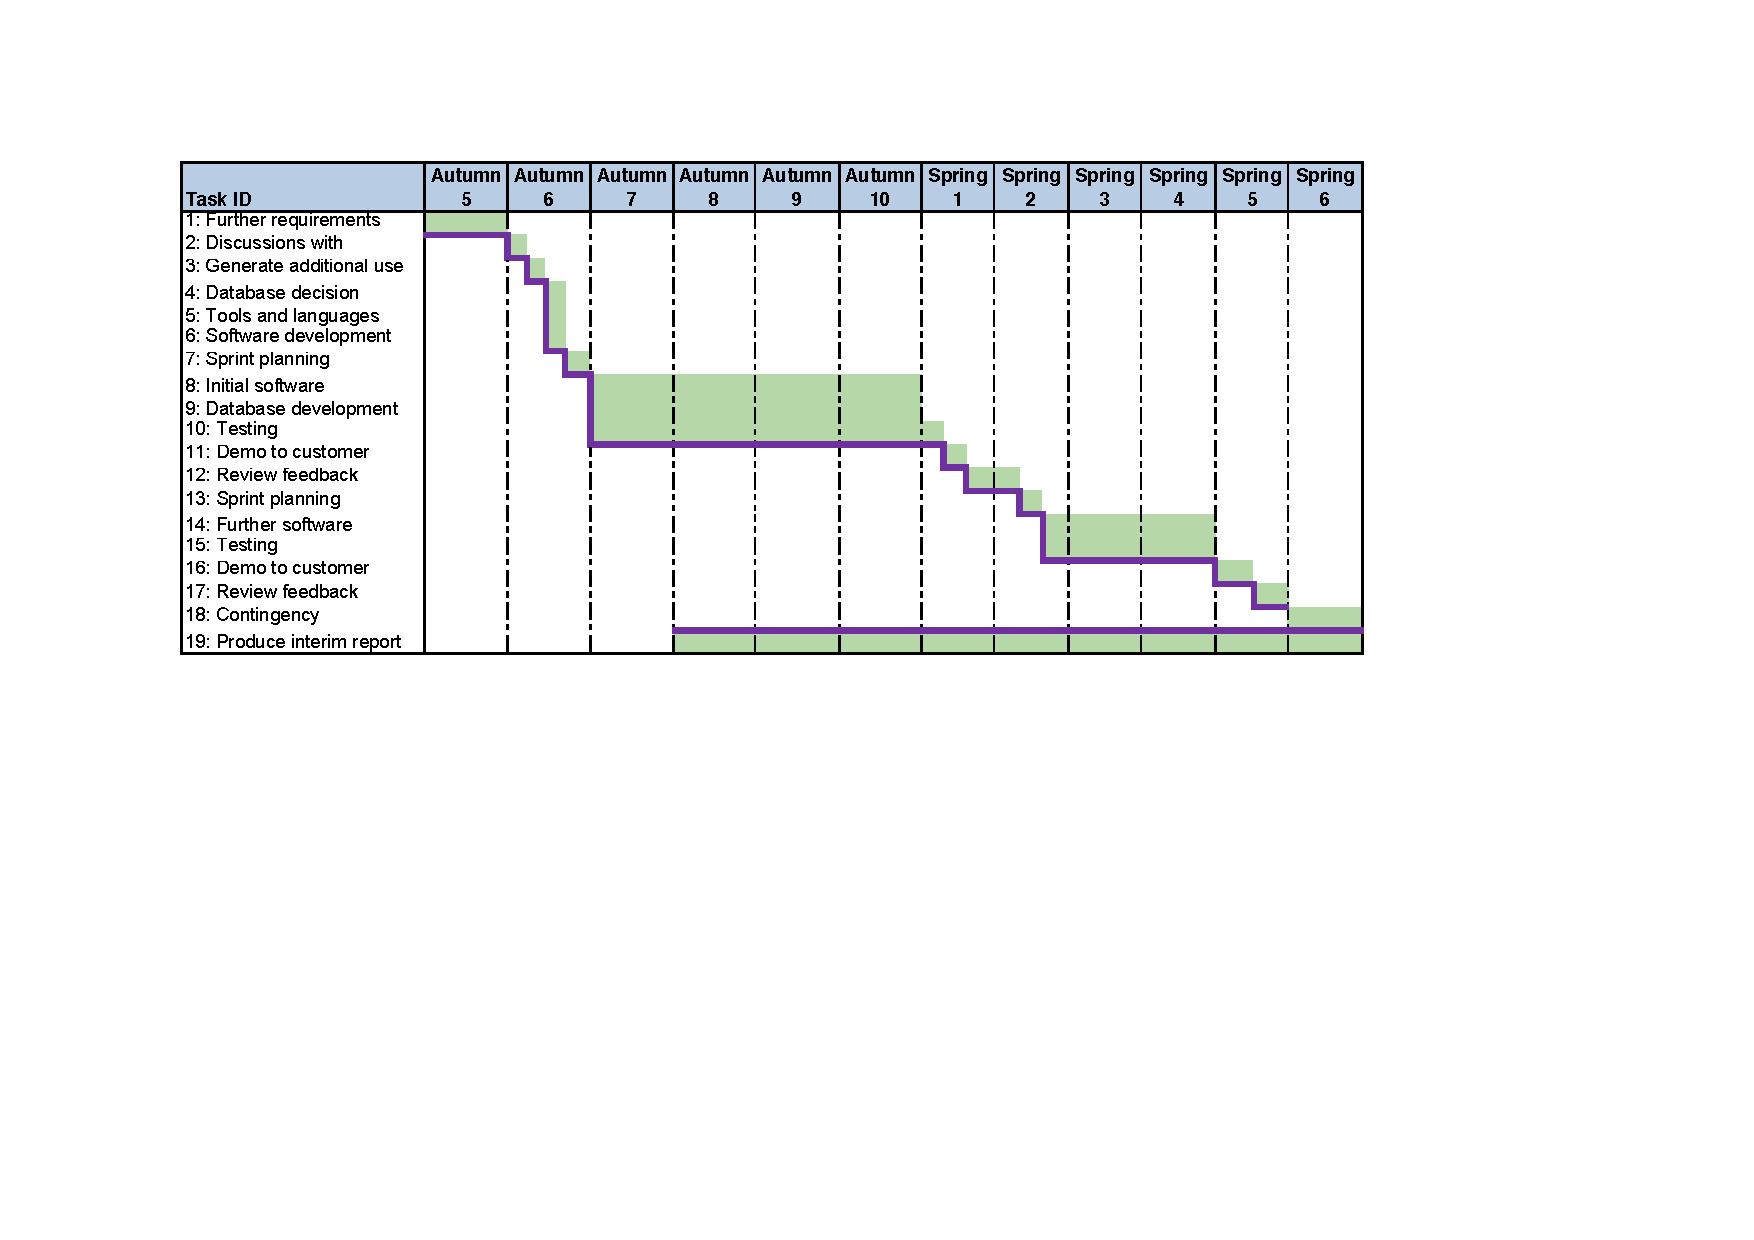
\includegraphics[width= 15cm]{images/GantInterim.pdf}
  \caption{Gantt chart for the interim phase of the project, purple shows the critical path.}
  \label{fig:ganttInterim}
\end{figure}

\begin{figure}[H]
  \centering
  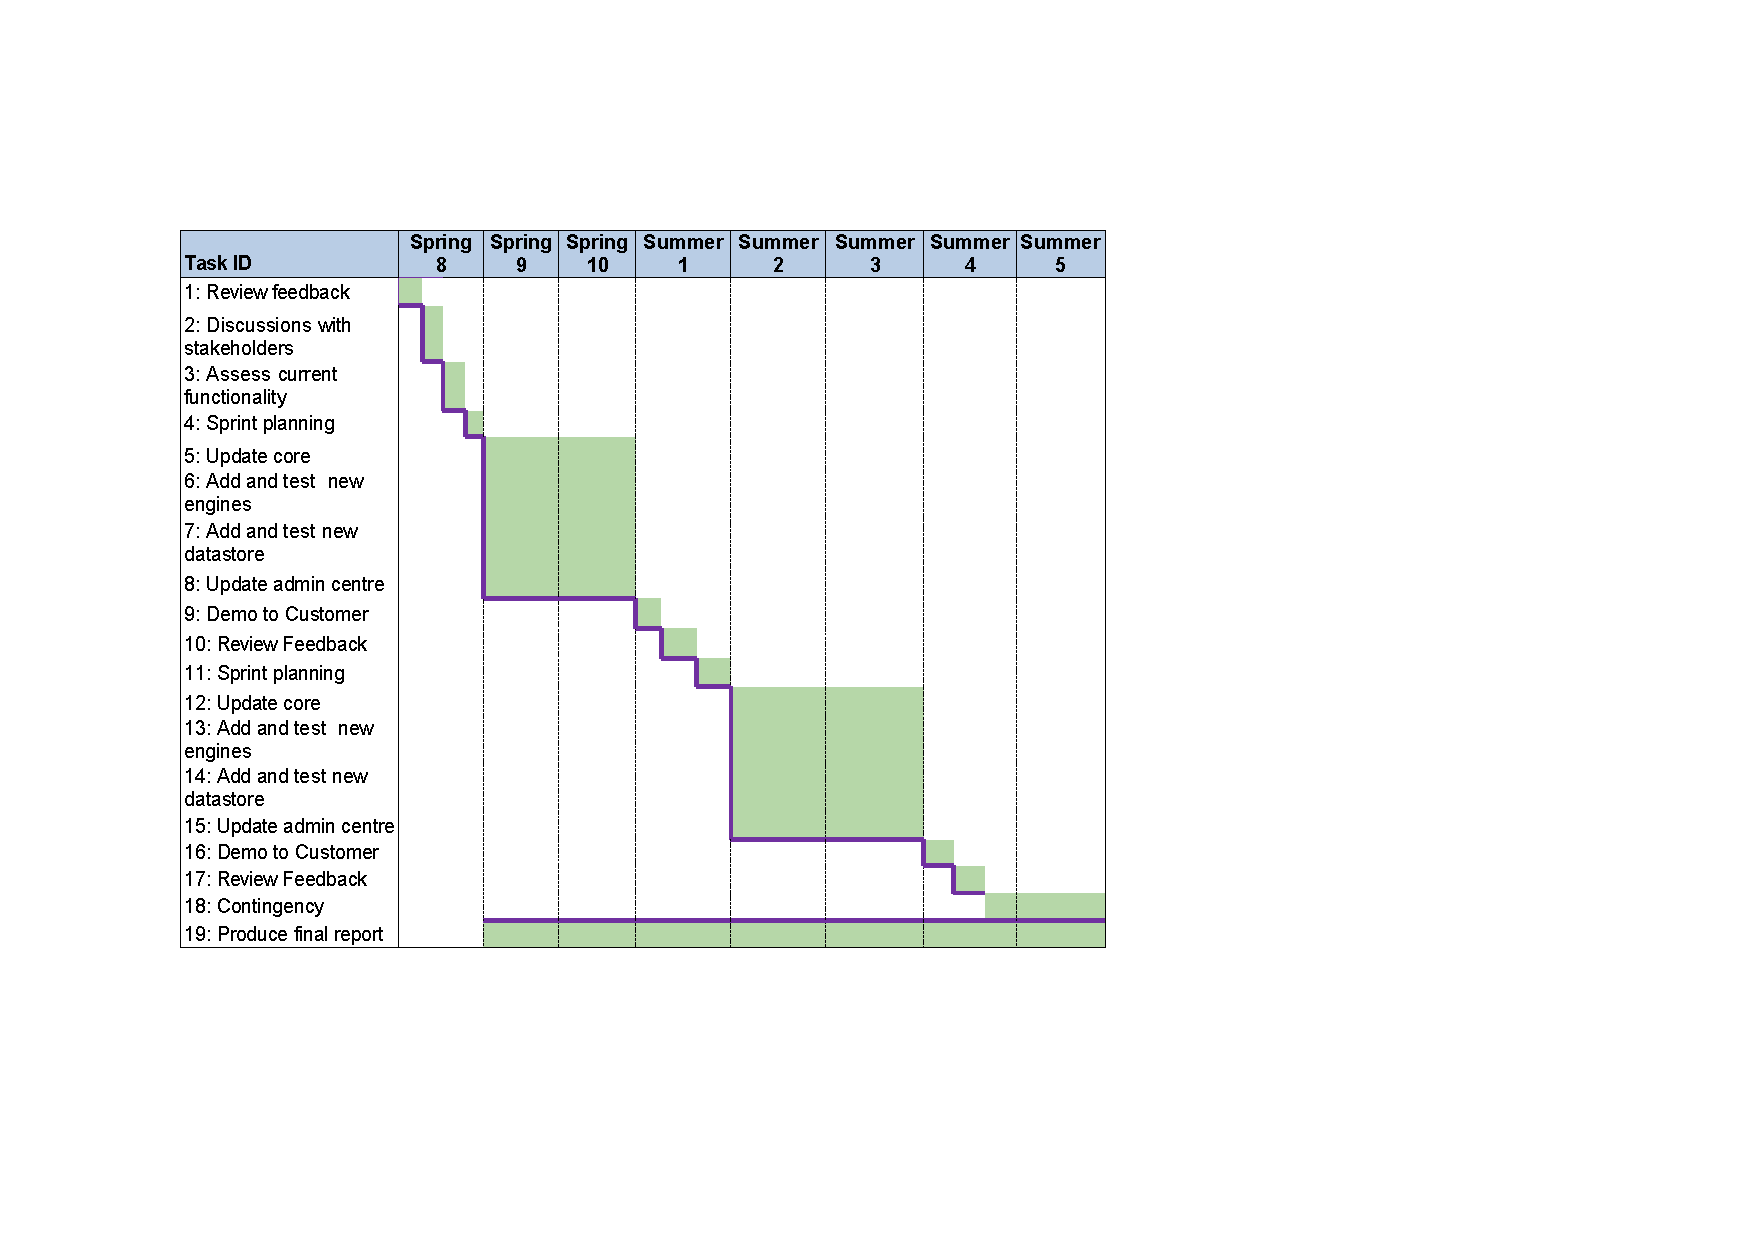
\includegraphics[width= 12cm]{images/GantFinal.pdf}
  \caption{Gantt chart for the final phase of the project, purple shows the critical path.}
  \label{fig:ganttFinal}
\end{figure}


% TODO - based on mark scheme!
% -> evidence that the risks have been considered in the planning of the development

\section{Risk register}
\label{sec:riskregister}

A risk assessment has been performed, based on design decisions made throughout the initial and interim phases of the project, ensuring team members are able to react to and correct problems when they occur. After feedback from the Customer, we took extra time to ensure both technical and procedural risks were identified early on. The risks from the Initial Report were reviewed and updated to reflect the more technical aspects of implementation. Risks relating to specific components were added, and some existing team planning risks were merged.

The hazards and risks have been identified by examining the 
current literature \cite{boehm1991software,jones1998minimizing}, drawing upon team members' past experiences and group discussion. Classification of the identified hazards, their impact on the system, and their probability of occurrence is performed in accordance with the Risk Management Guide for Information Technology Systems \cite{stoneburner2002risk}. The areas these hazards impact were then analysed, as well as the probability of occurrence. These are then weighted so that we can identify the risks which are likely to have the greatest detrimental effect on the project. The likelihood score (LS), impact score (IS), and risk matrix score (RS) are listed in the table below.

\begin{longtable}[H]{| p{0.6cm} | p{2.2cm} | p{0.26cm} | p{0.26cm} | p{2.7cm} | p{3cm} | p{2.6cm} | p{0.4cm} |}
  \hline
  \cellcolor{titleColor}\textbf{Risk ID} &
  \cellcolor{titleColor}\textbf{Risk} &
  \cellcolor{titleColor}\textbf{LS} &
  \cellcolor{titleColor}\textbf{IS} &
  \cellcolor{titleColor}\textbf{Impact Description} &
  \cellcolor{titleColor}\textbf{Mitigation} &
  \cellcolor{titleColor}\textbf{Contingency} &
  \cellcolor{titleColor}\textbf{RS}\\
  
  \hline \textbf{R.1}
  & Loss of team member(s).
  & 6
  & 3
  & Internal/external deadline failure.
  & Ensure all team project work is under version control.
 
  Use scrum methodology to proactively aid work reallocation, ensuring team members are aware of all assigned work.
  & Reallocate work across remaining team members, possibly notifying the customer and obtaining a deadline extension.
  & 18 \\
  
  \hline \textbf{R.2}
  & Team member(s) underperforming.
  & 6
  & 3
  & Internal/external deadline failure.
  & Identify team member strengths and weaknesses and assign work accordingly. 
  
  Build contingency time into the schedule to allow for underperformance.
  & Reallocate work across remaining team members, possibly notifying the customer and obtaining a deadline extension.
  & 18 \\
  
  \hline \textbf{R.3}
  & Time pressures limiting amount of development time.
  & 6
  & 4
  & Internal/external deadline failure.
  
  Not fulfilling requirements.
  
  Low quality deliverables.
  & Define scope of interim prototype early, commit to fulfilling requirements and allocate work to sprints.
  & Reduce functionality required and/or notify customer of later delivery.
  & 24 \\
  
  \hline \textbf{R.4}
  & Developed admin centre does not satisfy requirements.
  & 3
  & 3
  & Poor user experience.
  
  Loss of confidence in HUMS.
  & Continuous, iterative development process, regularly incorporating users feedback on the admin centre.
  & Redevelop admin centre.
  & 9\\
  
  \hline \textbf{R.5}
  & Deprecation of required Google App Engine functionality.
  & 3
  & 4

  & Unable to deliver required functionality.
  
  Loss of confidence in HUMS.
  & Research pending deprecations to ensure required functionality will be supported.
  & Migrate to another key-store database.
  & 12\\
  
  \hline \textbf{R.6}
  & Communic-ations link to Google App Engine fails.
  & 3
  & 4
  & Loss of service to users.

  Loss of confidence in the HUMS.
  & A final commercial version would use the premium Google service which guarantees an uptime of at least 99.95\% (\nfrit{9})
  & Additional data abstraction layer could be built to interface with another database service such as Heroku.
  & 12\\
  
  \hline \textbf{R.7}
  & Data interception between our application and Google App Engine.
  & 3
  & 2
  & Loss of confidence in the HUMS.
  & A final system would encrypt traffic between the HUMS and Google App Engine, currently just sending (non-sensitive) test data.
  & Additional penetration testing to identify security flaws.
  & 6\\
  
  \hline \textbf{R.8}
  & Data write/read times to and from Google App Engine are too slow.
  & 2
  & 5
  & Create a task backlog: gradual increase in load until system
  is non-operational.
  & Load test the HUMS throughout development.
  & Re-engineer HUMS, possibly switching datastore.
  & 10\\
  
  \hline \textbf{R.9}
  & HUMS does not facilitate data storage for a variety of systems.
  & 3
  & 5
  & Failure to meet key modifiability and flexibility requirements.
  & Adopt a key-value datastore allowing the flexibility to store a variety of data.
  & Examine difficult data and implement an additional SystemDataGateway,
  interfacing with a datastore capable of handling the data.
  & 15\\  
  
  \hline \textbf{R.10}
  & Included analysis components computing incorrect values.
  & 2
  & 5
  & Failing to meet fundamental requirements.
  
  Loss of confidence in the HUMS.
  & Adopt a test driven approach to development throughout the process
  ensuring expectations are met.
  & Re-engineer failing components.
  & 10\\
  
  \hline \textbf{R.11}
  & Included Analysis component computation too slow.
  & 3
  & 4
  & Creates an analysis task backlog: gradual increase in load until system
  is non-operational.
  & Load test analysis components throughout development.
  
    Optimise code.
  & Re-engineer analysis components.
  & 12\\  
  
  \hline \textbf{R.12}
  & Notification computation too slow.
  & 2
  & 4
  & Creates a notification backlog: gradual increase in load until system
  is non-operational.
  & Load test notification components throughout development.
 
  Optimise code.
  & Re-engineer notification system.
  & 8\\
  
  \hline \textbf{R.13}
  & GitHub becomes unavailable for a prolonged period of time.
  & 2
  & 2
  & Difficulty merging work from different machines.
  & Distributed nature of Git means little work would be lost.
  & Host our own Git server within the Computer Science Department.
  & 4\\ 
    \hline
\end{longtable}       

The likelihood score defines the probability of something occurring.
\textit{Kents Words of Estimative Probability}\cite{kent1966strategic} is utilised, with
`certain' weighted $7$ and `impossible' weighted $1$.

\begin{tabular}[H]{|p{1.45cm}|c|l|c|c|c|c|p{1.77cm}|}
  \cline{4-8} \multicolumn{3}{c|}{} & \multicolumn{5}{ c| }{Impact Score (Least$\rightarrow$Most)} \\
  \cline{4-8} \multicolumn{3}{c|}{} & 1 & 2 & 3 & 4 & 5 \\
  \cline{4-8} \multicolumn{3}{c|}{} & Negligible& Minor & Moderate& Major & Catastrophic \\

  \hline \multirow{7}{*}{Likelihood} & 7 & Certain & 7 & 14 & 21 & 28 & 35 \\

  \cline{2-8} & 6 & Almost certain & 6 & 12 & 18 & 24 & 30 \\
  \cline{2-8} & 5 & Probable& 5 & 10 & 15 & 20 & 25 \\
  \cline{2-8} & 4 & Chances about even & 4 & 8 & 12 & 16 & 20 \\
  \cline{2-8} & 3 & Probably not & 3 & 6 & 9 & 12 & 15 \\
  \cline{2-8} & 2 & Almost certainly not & 2 & 4 & 6 & 8 & 10 \\
  \cline{2-8} & 1 & Impossible & 1 & 2 & 3 & 4 & 5 \\
  \hline
\end{tabular}

\begin{longtable}[H]{ | p{2cm} | p{3cm} | p{8.5cm} | }
  \hline
  \cellcolor{titleColor}\textbf{Score} &
  \cellcolor{titleColor}\textbf{Risk Level} &
  \cellcolor{titleColor}\textbf{Recommended Response} \\

  \hline \textbf{23-35} & HIGH & Mitigation plan is
  required. Immediate action is required.\\

  \hline \textbf{11-22} & MEDIUM & To be included in the action plan
  and reviewed.\\

  \hline \textbf{0-10}& LOW & Included in action plan in limited
  scope. Minimum review. \\
  \hline
\end{longtable}


\section{Customer communication}
\label{sec:communication}

Our initial communication with the customer for this stage of the project was in the form of a face to face meeting where we received feedback on our previous report. This feedback was recorded and acted upon, including extending the risk register to include more technical risks and examining the qualities of the system. Our next contact was through email in which we sent a low fidelity prototype of the HUMS admin centre, explaining our idea of hosting a HUMS as a SaaS or PaaS, to which the customer replied the idea was interesting and suggested some small improvements. In response to this we worked on a new iteration of the admin centre and tweaked some of the information to better explain the HUMS concept and what a SaaS solution would offer.

After each communication with the customer we organised group meetings within two days to discuss the feedback issued and to collaborate on any improvements to our solution we could make based upon the feedback. In our next face to face meeting with the customer we explained our architectural ideas and discussed the test application, we then went on to have a team meeting where we planned how to monitor the test application. We then sent the customer a series of emails detailing implementation and architectural decisions, including the qualities and views we identified, and also an example of a reporting engine. The customer replied with helpful feedback, clarifying some of the qualities and including additional qualities they felt were important to the system, along with positive feedback on the module view diagram. We incoportated this feedback and additional information into our solution and report, and improved the reporting engine to show timestamps alongside data.


\vfill
\bibliography{report-refs}
\bibliographystyle{IEEEtran}
\end{document}
